% 一轮闯关训练 · 立体几何（题目 + 答案解析；图形全部为 TikZ 矢量图，源文件在 TikZ-final/geometry/solid）
% 一轮闯关训练 · 立体几何：本部分用到的小宏（elegantbook 已加载 pifont、xcolor）
% \bkstar{3}{5} → ★★★☆☆（难度）
\providecommand{\bkstar}[2]{{\color{main}\count255=0 \loop\ifnum\count255<#1 \ding{72}\advance\count255 by 1 \repeat}{\color{black!35}\count255=#1 \loop\ifnum\count255<#2 \ding{73}\advance\count255 by 1 \repeat}}
% \bktopic{异面直线所成角} → 小节里的题型标签
\providecommand{\bktopic}[1]{\par\medskip\noindent{\color{main}\bfseries ▍#1}\par\smallskip}
% 题号按讲重排：第 N 讲的练 k 显示为「题 N.k」，与原书一一对应（本部分位于讲义末尾，影响仅限于此）
\counterwithin*{exam}{section}
\renewcommand{\theexam}{\arabic{section}.\arabic{exam}}
% \bkfig[宽度]{TikZ-final/geometry/solid/pNNN-oNNNN.tex} → 居中插入矢量图
\providecommand{\bkfig}[2][0.25\textwidth]{\begin{figure}[H]\centering\resizebox{#1}{!}{\input{#2}}\end{figure}}


\section{第1讲\quad 空间几何体}
\subsection{夯基础}
\bktopic{构成空间几何体的基本元素及其关系}

\begin{example}[\bkstar{1}{5}]
如图中，点、直线、平面之间的关系用集合语言可表示为
\bkfig{TikZ-final/geometry/solid/p004-o0099.tex}
\begin{tasks}(1)
    \task $\alpha\cap\beta=m$，$n\subset\alpha$，$m\cap n=A$
    \task $\alpha\cap\beta=m$，$n\in\alpha$，$m\cap n=A$
    \task $\alpha\cap\beta=m$，$n\subset\alpha$，$A\subset m$，$A\subset n$
    \task $\alpha\cap\beta=m$，$n\in\alpha$，$A\in m$，$A\in n$
\end{tasks}
\end{example}
\begin{solution}
\textbf{答案：}A

由已知可得如图
\bkfig{TikZ-final/geometry/solid/p046-o0974.tex}
由图可知 $A$ 为点，$n$ 为直线，故可得 $n\subset\alpha$，则 $n\in\alpha$ 表示不正确，故排除B，D，而 $A\subset m$，$A\subset n$ 也表述不正确，故排除C，则A正确．

故选：A．
\end{solution}

\vspace{2em}

\bktopic{空间划分问题}

\begin{example}[\bkstar{2}{5}]
三个平面将空间最多能分成
\begin{tasks}(4)
    \task $6$ 部分
    \task $7$ 部分
    \task $8$ 部分
    \task $9$ 部分
\end{tasks}
\end{example}
\begin{solution}
\textbf{答案：}C

三个平面两两平行时，可以把空间分成 $4$ 部分；三个平面相交于同一条直线时，可以把空间分成 $6$ 部分；两个平面平行，第三个平面与它们相交时，可以把空间分成 $6$ 部分；三个平面两个相交，且交线互相平行时，可以把空间分成 $7$ 部分；三个平面两两相交，当三条不同的交线相交于一点时，可以把空间分成 $8$ 部分．所以空间中的三个平面最多能把空间分成 $8$ 部分．

故选：C．
\end{solution}

\vspace{2em}

\bktopic{棱锥的结构特征}

\begin{example}[\bkstar{2}{5}]
如图所示，观察四个几何体，其中判断正确的是
\begin{tasks}(4)
    \task \raisebox{-.5\height}{\resizebox{0.12\textwidth}{!}{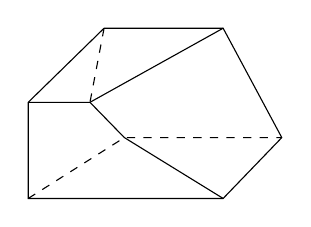
\begin{tikzpicture}[scale=.56]
  \coordinate (A) at (0,0); \coordinate (B) at (0,2.18);
  \coordinate (C) at (1.40,2.18); \coordinate (D) at (2.18,1.38);
  \coordinate (E) at (1.72,3.86); \coordinate (F) at (4.42,3.86);
  \coordinate (G) at (5.75,1.38); \coordinate (H) at (4.42,0);
  \draw (A)--(B)--(E)--(F)--(G)--(H)--cycle;
  \draw (B)--(C)--(D)--(H);
  \draw (C)--(F);
  \draw[dashed] (E)--(C) (A)--(D)--(G);
\end{tikzpicture}
}}\ 是棱台
    \task \raisebox{-.5\height}{\resizebox{0.08\textwidth}{!}{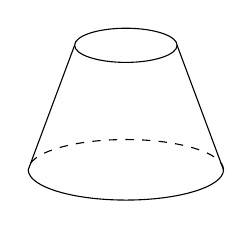
\begin{tikzpicture}[scale=.62]
  \draw (0,2.55) ellipse (1.05 and .35);
  \draw (-2,0) -- (-1.05,2.55) (2,0) -- (1.05,2.55);
  \draw (-2,0) arc[start angle=180,end angle=360,x radius=2,y radius=.62];
  \draw[dashed] (2,0) arc[start angle=0,end angle=180,x radius=2,y radius=.62];
\end{tikzpicture}
}}\ 是圆台
    \task \raisebox{-.5\height}{\resizebox{0.1\textwidth}{!}{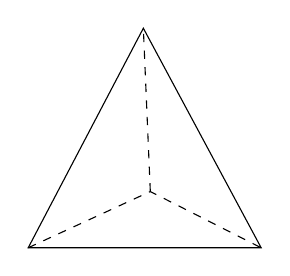
\begin{tikzpicture}[scale=.68]
  \coordinate (A) at (0,0); \coordinate (B) at (4.35,0);
  \coordinate (C) at (2.28,1.05); \coordinate (P) at (2.15,4.10);
  \draw (P)--(A)--(B)--cycle;
  \draw[dashed] (A)--(C)--(B) (C)--(P);
\end{tikzpicture}
}}\ 是棱锥
    \task \raisebox{-.5\height}{\resizebox{0.12\textwidth}{!}{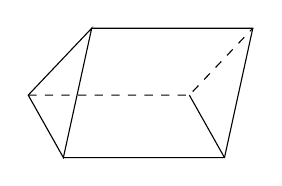
\begin{tikzpicture}[scale=.62]
  \coordinate (A) at (0,1.28); \coordinate (B) at (1.30,2.65);
  \coordinate (C) at (.72,0); \coordinate (D) at (3.30,1.28);
  \coordinate (E) at (4.60,2.65); \coordinate (F) at (4.02,0);
  \draw (A)--(B)--(C)--cycle;
  \draw (B)--(E)--(F)--(C);
  \draw (D)--(F);
  \draw[dashed] (A)--(D)--(E);
\end{tikzpicture}
}}\ 不是棱柱
\end{tasks}
\end{example}
\begin{solution}
\textbf{答案：}C

A．不满足棱台的定义，不正确；

B．不满足圆台的定义，不正确；

C．是棱锥，正确；

D．是棱柱，不正确．

故选：C．
\end{solution}

\vspace{2em}

\begin{example}[\bkstar{2}{5}]
将一个直角梯形绕其较短的底所在的直线旋转一周得到一个几何体，关于该几何体的以下描绘中，正确的是
\begin{tasks}(2)
    \task 是一个圆台
    \task 是一个圆柱
    \task 是一个圆柱和一个圆锥的简单组合体
    \task 是一个圆柱被挖去一个圆锥后所剩的几何体
\end{tasks}
\end{example}
\begin{solution}
\textbf{答案：}D

将一个直角梯形绕其较短的底所在的直线旋转一周得到一个圆柱被挖去一个圆锥后所剩的几何体．

故选：D．
\end{solution}

\vspace{2em}

\bktopic{多面体中的基础计算}

\begin{example}[\bkstar{2}{5}]
一个长方体的长、宽、高分别为 $3$，$4$，$5$，则这个长方体的体对角线长是
\begin{tasks}(4)
    \task $12$
    \task $10$
    \task $5\sqrt{2}$
    \task $2\sqrt{5}$
\end{tasks}
\end{example}
\begin{solution}
\textbf{答案：}C

由题意，长方体的体对角线长是 $\sqrt{9+16+25}=5\sqrt{2}$．

故选：C．
\end{solution}

\vspace{2em}

\begin{example}[\bkstar{2}{5}]
已知正四棱锥的底面边长为 $6$，高为 $4$，则斜高为
\begin{tasks}(4)
    \task $4$
    \task $3\sqrt{2}$
    \task $5$
    \task $4\sqrt{2}$
\end{tasks}
\end{example}
\begin{solution}
\textbf{答案：}C

如图
\bkfig[0.35\textwidth]{TikZ-final/geometry/solid/p047-o0996.tex}
$\because$ 正四棱锥 $P-ABCD$ 的底面边长为 $6$，$E$ 为 $AD$ 的中点，$O$ 为底面正方形的中心，

$\therefore OE=3$．

又正四棱锥的高 $PO=4$，所以斜高

$$
PE=\sqrt{PO^2+OE^2}=\sqrt{16+9}=5．
$$

故选：C．
\end{solution}

\vspace{2em}

\bktopic{表面积与体积}

\begin{example}[\bkstar{2}{5}]
一个高为 $2$ 的圆柱，底面周长为 $2\pi$，该圆柱的表面积为
\end{example}
\begin{solution}
\textbf{答案：}$6\pi$

因为一个高为 $2$ 的圆柱，底面周长为 $2\pi$，所以它的底面半径为 $1$，所以圆柱的表面积为

$$
S=2S_{\text{底}}+S_{\text{侧}}=2\times 1^2\times\pi+2\pi\times 2=6\pi．
$$

故答案为：$6\pi$．
\end{solution}

\vspace{2em}

\begin{example}[\bkstar{2}{5}]
圆锥的底面半径为 $1$，高为 $\sqrt{3}$，则圆锥的表面积为
\begin{tasks}(4)
    \task $\pi$
    \task $2\pi$
    \task $3\pi$
    \task $4\pi$
\end{tasks}
\end{example}
\begin{solution}
\textbf{答案：}C

圆锥的底面半径为 $1$，高为 $\sqrt{3}$，则母线长 $l=\sqrt{1^2+\left(\sqrt{3}\right)^2}=2$，圆锥的表面积

$$
S=S_{\text{底面}}+S_{\text{侧面}}=\pi r^2+\pi rl=\pi+2\pi=3\pi．
$$

故选：C．
\end{solution}

\vspace{2em}

\bktopic{球}

\begin{example}[\bkstar{2}{5}]
半径为 $2$ 的球的表面积为
\begin{tasks}(4)
    \task $4\pi$
    \task $8\pi$
    \task $12\pi$
    \task $16\pi$
\end{tasks}
\end{example}
\begin{solution}
\textbf{答案：}D

$\because$ 球的半径 $R=2$，

$\therefore$ 球的表面积为 $4\pi\times R^2=4\pi\times 4=16\pi$．

故选：D．
\end{solution}

\vspace{2em}

\begin{example}[\bkstar{1}{5}]
已知球的半径为 $1$，则该球的体积是
\begin{tasks}(4)
    \task $\dfrac{4}{3}$
    \task $\pi$
    \task $\dfrac{4\pi}{3}$
    \task $4\pi$
\end{tasks}
\end{example}
\begin{solution}
\textbf{答案：}C

由球的体积公式得 $V=\dfrac{4\pi}{3}$．

故选：C．
\end{solution}

\vspace{2em}

\subsection{刷中档}
\bktopic{棱锥的结构特征}

\begin{example}[\bkstar{2}{5}]
若一个棱锥的各棱长均相等，则该棱锥一定不是
\begin{tasks}(4)
    \task 三棱锥
    \task 四棱锥
    \task 五棱锥
    \task 六棱锥
\end{tasks}
\end{example}
\begin{solution}
\textbf{答案：}D

若一个棱锥的各棱长均相等，则该棱锥一定不是六棱锥．因为正六边形的顶点到中心的距离等于边长，所以正六棱锥的侧棱必大于底面棱长．

故选：D．
\end{solution}

\vspace{2em}

\begin{example}[\bkstar{2}{5}]
某人用如图所示的纸片，沿折痕折后粘成一个四棱锥形的“走马灯”，正方形做灯底，且有一个三角形面上写上了“福”字，当灯逆时针旋转时，正好看到“幸福芜湖”的字样，则在①②③处可以依次写上
\bkfig[0.2\textwidth]{TikZ-final/geometry/solid/p006-o0134.tex}
\begin{tasks}(1)
    \task 芜、幸、湖
    \task 湖、幸、芜
    \task 幸、芜、湖
    \task 湖、芜、幸
\end{tasks}
\end{example}
\begin{solution}
\textbf{答案：}C

画出图形，如图所示．
\bkfig[0.3\textwidth]{TikZ-final/geometry/solid/p049-o1025.tex}
根据四棱锥图形，正好看到“幸福芜湖”的字样，可知顺序为①福②③，则在①②③处可以依次写上幸、芜、湖．

故选：C．
\end{solution}

\vspace{2em}

\begin{example}[\bkstar{2}{5}]
下列各图都是正方体的表面展开图，将其还原成正方体后，所得正方体完全一致（数码相对位置相同）的是
\bkfig[0.6\textwidth]{TikZ-final/geometry/solid/p007-o0147.tex}
\begin{tasks}(4)
    \task （Ⅰ）和（Ⅳ）
    \task （Ⅰ）和（Ⅲ）
    \task （Ⅱ）和（Ⅲ）
    \task （Ⅱ）和（Ⅳ）
\end{tasks}
\end{example}
\begin{solution}
\textbf{答案：}B

（Ⅰ）图还原后，①④对面，②⑤对面，③⑥对面；

（Ⅱ）图还原后，①⑥对面，②⑤对面，③④对面；

（Ⅲ）图还原后，①④对面，②⑤对面，③⑥对面；

（Ⅳ）图还原后，①⑤对面，②④对面，③⑥对面．

综上，可得还原成正方体后，其中两个完全一样的是（Ⅰ）和（Ⅲ）．

故选：B．
\end{solution}

\vspace{2em}

\begin{example}[\bkstar{3}{5}]
正方体的直观图如图所示，则其展开图是（要求把可能的序号都填上）．
\bkfig[0.45\textwidth]{TikZ-final/geometry/solid/p007-o0148.tex}
\end{example}
\begin{solution}
\textbf{答案：}(4)

根据题意，可得：

对于（1），展开图中的上下两边的正方形的对边中点连线应该呈左右方向显现，故（1）的图形不符合题意；

对于（2），展开图中最右边的“日”字形正方形的对边中点连线应该是上下方向呈现，且应该在含有圆形的正方形的左边放置，故（2）的图形不符合题意；

对于（3），展开图中最右边的正方形应该与含有圆形的正方形相邻，故（3）的图形不符合题意；

对于（4），沿如图的红线将正方体的侧面剪裁，展开可得如（4）图的形状，故（4）的图形符合题意．
\bkfig{TikZ-final/geometry/solid/p050-o1038.tex}
故答案为：（4）．
\end{solution}

\vspace{2em}

\bktopic{表面积与体积}

\begin{example}[\bkstar{3}{5}]
如图所示，三棱柱 $ABC-A_1B_1C_1$ 的体积为 $6$．$O$ 为四边形 $BCC_1B_1$ 的中心，则四面体 $A_1-B_1OB$ 的体积为
\bkfig[0.3\textwidth]{TikZ-final/geometry/solid/p007-o0153.tex}
\end{example}
\begin{solution}
\textbf{答案：}$1$

如图，连接 $A_1C$，$B_1C$．
\bkfig[0.3\textwidth]{TikZ-final/geometry/solid/p050-o1043.tex}
在三棱柱 $ABC-A_1B_1C_1$ 中，$V_{A_1-BB_1C}=V_{A_1-B_1C_1C}$，而 $V_{A_1-BB_1C}=V_{C-A_1B_1B}=V_{C-AA_1B}$，

$\therefore$ 四面体 $A_1-B_1BC$ 的体积 $V=\dfrac{1}{3}V_{ABC-A_1B_1C_1}=\dfrac{1}{3}\times 6=2$，

则四面体 $A_1-B_1OB$ 的体积为 $\dfrac{1}{2}V_{A_1-BB_1C}=\dfrac{1}{2}\times 2=1$．

故答案为：$1$．
\end{solution}

\vspace{2em}

\begin{example}[\bkstar{2}{5}]
设三棱锥 $P-ABC$ 的三条侧棱两两垂直，且满足 $PA=PB=PC=1$，则三棱锥 $P-ABC$ 的体积是
\end{example}
\begin{solution}
\textbf{答案：}$\dfrac{1}{6}$

因为三棱锥 $P-ABC$ 的三条侧棱两两垂直，且 $PA=PB=PC=1$，所以由题意可知，三棱锥 $P-ABC$ 的体积：

$$
V_{P-ABC}=V_{A-PBC}=\dfrac{1}{3}\times\dfrac{1}{2}\times 1\times 1\times 1=\dfrac{1}{6}．
$$

故答案为：$\dfrac{1}{6}$．
\end{solution}

\vspace{2em}

\begin{example}[\bkstar{3}{5}]
在正三棱柱 $ABC-A_1B_1C_1$ 中，各侧棱和底面的边长均为 $a$，点 $D$ 是 $CC_1$ 上任意一点，连接 $A_1B$，$BD$，$A_1D$，$AD$，则三棱锥 $A-A_1BD$ 的体积为
\begin{tasks}(4)
    \task $\dfrac{1}{6}a^3$
    \task $\dfrac{\sqrt{3}}{12}a^3$
    \task $\dfrac{\sqrt{3}}{6}a^3$
    \task $\dfrac{1}{12}a^3$
\end{tasks}
\end{example}
\begin{solution}
\textbf{答案：}B
\bkfig[0.3\textwidth]{TikZ-final/geometry/solid/p050-o1044.tex}
由题意可知，

$$
V_{A-A_1BD}=V_{D-A_1BA}=\dfrac{1}{3}\times\dfrac{a^2}{2}\times\dfrac{\sqrt{3}a}{2}=\dfrac{\sqrt{3}a^3}{12}．
$$

故选：B．
\end{solution}

\vspace{2em}

\bktopic{球}

\begin{example}[\bkstar{3}{5}]
如图，有一个水平放置的透明无盖的正方体容器，容器高 $4\,\mathrm{cm}$，将一个球放在容器口，再向容器内注水，当球面恰好接触水面时测得水深为 $3\,\mathrm{cm}$，如果不计容器的厚度，则球的体积为
\bkfig[0.22\textwidth]{TikZ-final/geometry/solid/p008-o0171.tex}
\begin{tasks}(1)
    \task $\dfrac{125\pi}{6}\,\mathrm{cm}^3$
    \task $\dfrac{433\pi}{6}\,\mathrm{cm}^3$
    \task $\dfrac{343\pi}{6}\,\mathrm{cm}^3$
    \task $\dfrac{256\pi}{6}\,\mathrm{cm}^3$
\end{tasks}
\end{example}
\begin{solution}
\textbf{答案：}A

设球的半径为 $R$，设正方体上底面截球所得截面圆恰好为上底面正方形的内切圆，该圆的半径为 $r=2\,\mathrm{cm}$，且该截面圆圆心到水面的距离为 $1\,\mathrm{cm}$，即球心到截面圆圆心的距离为 $(R-1)\,\mathrm{cm}$．

由勾股定理可得 $R^2=(R-1)^2+2^2$，解得 $R=\dfrac{5}{2}\,\mathrm{cm}$．

因此，球的体积为

$$
\dfrac{4}{3}\pi R^3=\dfrac{4}{3}\pi\times\left(\dfrac{5}{2}\right)^3=\dfrac{125\pi}{6}\,\mathrm{cm}^3．
$$

故选：A．
\end{solution}

\vspace{2em}

\bktopic{旋转体表面的最短路径问题}

\begin{example}[\bkstar{3}{5}]
如图，圆锥的主视图是等边三角形，圆锥的底面半径为 $2\,\mathrm{cm}$．若点 $B$ 有一只蚂蚁只能沿圆锥的表面爬行，它要想吃到母线 $AC$ 的中点 $P$ 处的食物，那么它爬行的最短路程是（\qquad）$\mathrm{cm}$
\bkfig[0.2\textwidth]{TikZ-final/geometry/solid/p008-o0172.tex}
\begin{tasks}(1)
    \task $6$
    \task $2\sqrt{5}$
    \task $4$
    \task $\sqrt{5}$
\end{tasks}
\end{example}
\begin{solution}
\textbf{答案：}B

由题意，圆锥底面半径为 $2\,\mathrm{cm}$，母线长为 $4\,\mathrm{cm}$，则展开后所得扇形的半径为 $4\,\mathrm{cm}$，弧长为 $4\pi\,\mathrm{cm}$，则展开后所得扇形的圆心角为 $\pi$．

如图
\bkfig[0.3\textwidth]{TikZ-final/geometry/solid/p051-o1057.tex}
$\because AB=4\,\mathrm{cm}$，$AP=2\,\mathrm{cm}$，

$\therefore BP=\sqrt{4^2+2^2}=2\sqrt{5}\,\mathrm{cm}$．

故选：B．
\end{solution}

\vspace{2em}

\begin{example}[\bkstar{3}{5}]
如图所示的圆柱的底面圆半径为 $1$，四边形 $ABCD$ 为圆柱的轴截面，从 $A$ 点出发沿着圆柱的侧面拉一条绳子到 $C$ 点，若绳子的最短长度为 $3\pi$，则该圆柱的侧面积为
\bkfig[0.18\textwidth]{TikZ-final/geometry/solid/p009-o0185.tex}
\end{example}
\begin{solution}
\textbf{答案：}$4\sqrt{2}\pi^2$

将圆柱的侧面沿 $AD$ 展开，绳子的最短长度即展开后 $A$，$C$ 两点间的距离，连接 $AC$，则 $AC=3\pi$．易知展开后 $AB$ 的长度为 $\pi$，设圆柱的高为 $h$，则 $AC^2=AB^2+h^2$，即 $9\pi^2=h^2+\pi^2$，所以 $h=2\sqrt{2}\pi$．

所以圆柱的侧面积为 $2\times\pi\times 2\sqrt{2}\pi=4\sqrt{2}\pi^2$．

故答案为：$4\sqrt{2}\pi^2$．
\end{solution}

\vspace{2em}

\subsection{提能力}
\bktopic{多面体中的截面分析}

\begin{example}[\bkstar{3}{5}]
正方体 $ABCD-A_1B_1C_1D_1$ 中，$P$，$Q$，$R$ 分别是 $AB$，$AD$，$B_1C_1$ 的中点．那么，正方体过 $P$，$Q$，$R$ 的截面图形是
\begin{tasks}(4)
    \task 三角形
    \task 四边形
    \task 五边形
    \task 六边形
\end{tasks}
\end{example}
\begin{solution}
\textbf{答案：}D
\bkfig[0.3\textwidth]{TikZ-final/geometry/solid/p052-o1072.tex}
通过画图，可以得到这个截面与正方体的六个面都相交，所以截面为六边形．

故选：D．
\end{solution}

\vspace{2em}

\begin{example}[\bkstar{3}{5}]
正方体的截面不可能是：
\begin{enumerate}
    \item[①] 钝角三角形；
    \item[②] 直角三角形；
    \item[③] 菱形；
    \item[④] 正五边形；
    \item[⑤] 正六边形．
\end{enumerate}
下述选项正确的是
\begin{tasks}(4)
    \task ①②⑤
    \task ①②④
    \task ②③④
    \task ③④⑤
\end{tasks}
\end{example}
\begin{solution}
\textbf{答案：}B

若截面为三角形 $ABC$，$OA=a$，$OB=b$，$OC=c$，$AC^2=a^2+c^2$，$AB^2=a^2+b^2$，$BC^2=b^2+c^2$，

$$
\therefore \cos\angle CAB=\dfrac{AB^2+AC^2-BC^2}{2AB\cdot AC}=\dfrac{2a^2}{2\sqrt{a^2+b^2}\sqrt{a^2+c^2}}>0，
$$

$\therefore \angle CAB$ 为锐角，同理 $\angle ACB$ 与 $\angle ABC$ 也为锐角，即 $\triangle ABC$ 为锐角三角形；

取正方体相对棱的中点，得到的四边形是菱形；

正方体有六个面，用平面去截正方体时最多与六个面相交得六边形为正六边形；

经过正方体的一个顶点去切就可得到五边形，但此时不可能是正五边形．

故不可能是①②④．

故选：B．
\end{solution}

\vspace{2em}

\bktopic{表面积与体积}

\begin{example}[\bkstar{3}{5}]
圆柱的底面直径和母线长均为 $2$，则此圆柱的外接球的表面积为
\begin{tasks}(4)
    \task $\dfrac{8}{3}\pi$
    \task $\dfrac{8\sqrt{2}}{3}\pi$
    \task $4\pi$
    \task $8\pi$
\end{tasks}
\end{example}
\begin{solution}
\textbf{答案：}D

圆柱的底面半径与母线的一半都是 $1$，圆柱外接球的半径为：$\sqrt{1^2+1^2}=\sqrt{2}$，圆柱的外接球的表面积为：$4\pi\left(\sqrt{2}\right)^2=8\pi$．

故选：D．
\end{solution}

\vspace{2em}

\begin{example}[\bkstar{3}{5}]
已知球 $O$ 与正方体各棱均相切，若正方体棱长为 $\sqrt{2}$，则球 $O$ 的表面积为
\begin{tasks}(4)
    \task $\dfrac{4\pi}{3}$
    \task $2\pi$
    \task $4\pi$
    \task $6\pi$
\end{tasks}
\end{example}
\begin{solution}
\textbf{答案：}C

球 $O$ 与正方体各棱均相切，正方体棱长为 $\sqrt{2}$，则球 $O$ 的半径为

$$
R=\dfrac{\sqrt{\left(\sqrt{2}\right)^2+\left(\sqrt{2}\right)^2}}{2}=1，
$$

所以球 $O$ 的表面积为 $4\pi R^2=4\pi\times 1=4\pi$．

故选：C．
\end{solution}

\vspace{2em}

\bktopic{多面体表面的最短路径问题}

\begin{example}[\bkstar{3}{5}]
如图，直三棱柱 $ABC-A_1B_1C_1$ 中，$AB=AC=1$，$AA_1=2$，$F$ 为线段 $AA_1$ 上的一动点，则 $BF+FC_1$ 的最小值为
\bkfig[0.18\textwidth]{TikZ-final/geometry/solid/p010-o0199.tex}
\begin{tasks}(1)
    \task $1$
    \task $2\sqrt{2}$
    \task $\sqrt{2}$
    \task $\sqrt{3}$
\end{tasks}
\end{example}
\begin{solution}
\textbf{答案：}B

将侧面 $ABB_1A_1$ 和侧面 $ACC_1A_1$ 沿 $AA_1$ 展到一个平面内，如下图
\bkfig[0.3\textwidth]{TikZ-final/geometry/solid/p053-o1086.tex}
连接平面图中 $BC_1$，交 $AA_1$ 于点 $F$，此时可使 $BF+FC_1$ 取得最小值，为平面图中线段 $BC_1$ 的长．

$\because AB=AC=1$，$AA_1=2$，

在直三棱柱 $ABC-A_1B_1C_1$ 中，有 $CC_1=AA_1=2$，且 $CC_1\perp AC$，

$\therefore$ 由勾股定理得：平面图中线段 $BC_1=\sqrt{2^2+2^2}=2\sqrt{2}$，

即 $BF+FC_1$ 的最小值为 $2\sqrt{2}$．

故选：B．
\end{solution}

\vspace{2em}

\begin{example}[\bkstar{3}{5}]
如图，$M$ 是棱长为 $2$ 的正方体 $ABCD-A_1B_1C_1D_1$ 的棱 $CC_1$ 的中点，沿正方体表面从点 $A$ 到点 $M$ 的最短路程是
\bkfig[0.22\textwidth]{TikZ-final/geometry/solid/p010-o0200.tex}
\end{example}
\begin{solution}
\textbf{答案：}$\sqrt{13}$

由题意，若以 $BC$，$DC$ 为轴展开，则以 $AM$ 两点连成的线段为斜边所构成的直角三角形的两直角边的长度分别为 $2$，$3$，故两点之间的距离是 $\sqrt{13}$；

若以 $BB_1$ 为轴展开，则以 $AM$ 两点连成的线段为斜边所构成的直角三角形的两直角边的长度分别为 $1$，$4$，故两点之间的距离是 $\sqrt{17}$．

故沿正方体表面从点 $A$ 到点 $M$ 的最短路程是 $\sqrt{13}$．

故答案为：$\sqrt{13}$．
\end{solution}

\vspace{2em}

\section{第2讲\quad 空间中的平行关系}
\subsection{夯基础}
\bktopic{点、线确定平面}

\begin{example}[\bkstar{2}{5}]
下列四个条件中，能确定一个平面的条件是
\begin{tasks}(4)
    \task 空间任意三点
    \task 空间两条直线
    \task 空间两条平行直线
    \task 一条直线和一个点
\end{tasks}
\end{example}
\begin{solution}
\textbf{答案：}C

A．当这三个点共线时经过这三点的平面有无数个，故A错

B．当这两条直线是异面直线时，则根据异面直线的定义可得这对异面直线不同在任何一个平面内，故B错

C．根据确定平面的公理的推论可知两条平行直线可唯一确定一个平面，故C对

D．此点在此直线上时有无数个平面经过这条直线和这个点，故D错

故选：C．
\end{solution}

\vspace{2em}

\begin{example}[\bkstar{2}{5}]
空间四点最多可确定平面的个数是
\begin{tasks}(4)
    \task $1$
    \task $2$
    \task $3$
    \task $4$
\end{tasks}
\end{example}
\begin{solution}
\textbf{答案：}D

根据题意知，空间四点确定的直线的位置关系有三种

\ding{172}当空间四点确定的两条直线平行或相交或有且只有三点共线时，则四个点确定 $1$ 个平面

\ding{173}当空间四点确定的两条直线异面时，四点不共面，如三棱锥的顶点和底面上的顶点，则四个点确定 $4$ 个平面

\ding{174}当空间四点在一条直线上时，可确定 $0$ 个平面

故空间四点最多可确定 $4$ 个平面

故选：D．
\end{solution}

\vspace{2em}

\bktopic{直线与平面平行}

\begin{example}[\bkstar{1}{5}]
直线 $l\px\alpha$，在 $\alpha$ 内与 $l$ 平行的直线
\begin{tasks}(4)
    \task 有 $1$ 条
    \task 有 $2$ 条
    \task 有无数条
    \task 不可能有无数条
\end{tasks}
\end{example}
\begin{solution}
\textbf{答案：}C

直线 $l\px\alpha$

则平面 $\alpha$ 内必有一条直线 $m$ 与 $l$ 平行

平面 $\alpha$ 内有无数条直线与 $m$ 平行

则平面 $\alpha$ 内与 $l$ 平行的直线有无数条

故选：C．
\end{solution}

\vspace{2em}

\begin{example}[\bkstar{2}{5}]
在正方体 $ABCD-A_1B_1C_1D_1$ 中，$H$，$E$，$F$，$G$ 分别为 $DC$，$BB_1$，$AA_1$，$CC_1$ 的中点，则与平面 $HFE$ 平行的直线是
\begin{tasks}(4)
    \task $B_1G$
    \task $BD$
    \task $A_1C_1$
    \task $B_1C$
\end{tasks}
\end{example}
\begin{solution}
\textbf{答案：}A

\bkfig{TikZ-final/geometry/solid/p055-o1140.tex}
连接 $B_1G$，$CE$，$FD$

把平面 $HEF$ 延展成平面 $CDFE$

$\because E$，$G$ 分别是 $B_1B$，$C_1C$ 的中点

$\therefore B_1G\px CE$

又 $CE\subset$ 平面 $CDFE$，$B_1G\not\subset$ 平面 $CDFE$

$\therefore B_1G\px$ 平面 $CDFE$

故而 $B_1G\px$ 平面 $HFE$

故选：A．
\end{solution}

\vspace{2em}

\begin{example}[\bkstar{1}{5}]
在正方体 $ABCD-A_1B_1C_1D_1$ 中，$E$ 为 $DD_1$ 的中点，则下列直线中与平面 $ACE$ 平行的是
\begin{tasks}(4)
    \task $BA_1$
    \task $BD_1$
    \task $BC_1$
    \task $BB_1$
\end{tasks}
\end{example}
\begin{solution}
\textbf{答案：}B

\bkfig{TikZ-final/geometry/solid/p055-o1142.tex}
如图，连接 $BD$，与 $AC$ 交于 $O$ 点，则 $O$ 是 $BD$ 中点，连接 $OE$，$BD_1$

又 $\because E$ 为 $DD_1$ 的中点

$\therefore OE\px BD_1$

$\because OE\subset$ 平面 $ACE$，$BD_1\not\subset$ 平面 $ACE$

$\therefore BD_1\px$ 平面 $ACE$

故选：B．
\end{solution}

\vspace{2em}

\begin{example}[\bkstar{1}{5}]
在正方体 $ABCD-A_1B_1C_1D_1$ 中，$M$ 是棱 $CD$ 上的动点，则直线 $MC_1$ 与平面 $AA_1B_1B$ 的位置关系是
\bkfig{TikZ-final/geometry/solid/p012-o0261.tex}
\begin{tasks}(1)
    \task 相交
    \task 平行
    \task 异面
    \task 相交或平行
\end{tasks}
\end{example}
\begin{solution}
\textbf{答案：}B

$\because MC_1\subset$ 平面 $DD_1C_1C$，平面 $AA_1B_1B\px$ 平面 $DD_1C_1C$

$\therefore MC_1\px$ 平面 $AA_1B_1B$

故选：B．
\end{solution}

\vspace{2em}

\begin{example}[\bkstar{2}{5}]
如图，在四棱锥 $P-ABCD$ 中，平面 $PAD\perp$ 平面 $ABCD$，$AB=AD$，$\angle BAD=60^{\circ}$，$E$，$F$ 分别是 $AP$，$AD$ 的中点，求证：直线 $EF\px$ 平面 $PCD$；
\bkfig{TikZ-final/geometry/solid/p012-o0262.tex}
\end{example}
\begin{solution}
在 $\triangle PAD$ 中，因为 $E$，$F$ 分别为 $AP$，$AD$ 的中点

所以 $EF\px PD$

又因为 $EF$ 不在平面 $PCD$ 中，$PD\subset$ 平面 $PCD$

所以直线 $EF\px$ 平面 $PCD$ % 待核对：原书此行末尾多印“PAD”，疑为排版残留，已略去
\end{solution}

\vspace{2em}

\bktopic{平面与平面平行}

\begin{example}[\bkstar{2}{5}]
在正方体 $EFGH-E_1F_1G_1H_1$ 中，平面 $E_1FG_1$ 与平面 $EGH_1$，平面 $FHG_1$ 与平面 $F_1H_1G$，平面 $F_1H_1H$ 与平面 $FHE_1$，平面 $E_1HG_1$ 与平面 $EH_1G$ 中互相平行的对数为
\begin{tasks}(4)
    \task $0$
    \task $1$
    \task $2$
    \task $3$
\end{tasks}
\end{example}
\begin{solution}
\textbf{答案：}B

由图形易得 $E_1F\px H_1G$，$EG\px E_1G_1$，$E_1F\cap E_1G_1=E_1$，$H_1G\cap EG=G$，从而易得平面 $E_1FG_1\px$ 平面 $EGH_1$

在平面 $FHG_1$ 中，$F_1G$ 与 $FG_1$ 相交，则平面 $FHG_1$ 与平面 $F_1H_1G$ 相交

$HH_1\cap FH=H$，则平面 $F_1H_1H$ 与平面 $FHE_1$ 相交

在平面 $EH_1G$ 中，$EH_1$ 与 $E_1H$ 相交，平面 $E_1HG_1$ 与平面 $EH_1G$ 相交

故选：B．
\end{solution}

\vspace{2em}

\begin{example}[\bkstar{2}{5}]
如图所示，在直四棱柱 $ABCD-A_1B_1C_1D_1$ 中，$A_1A=2$，底面是边长为 $1$ 的正方形，$E$，$F$，$G$ 分别是棱 $BB_1$，$AA_1$，$AD$ 的中点，则平面 $A_1DE$ 与平面 $BGF$ 的位置关系是（填“平行”或“相交”）．
\bkfig{TikZ-final/geometry/solid/p013-o0283.tex}
\end{example}
\begin{solution}
\textbf{答案：}平行

\bkfig{TikZ-final/geometry/solid/p056-o1163.tex}
$\because$ 在直四棱柱 $ABCD-A_1B_1C_1D_1$ 中，$A_1A=2$，底面是边长为 $1$ 的正方形

$E$，$F$，$G$ 分别是棱 $BB_1$，$AA_1$，$AD$ 的中点

$\therefore FG\px A_1D$，$A_1F\px BE$

$\therefore$ 四边形 $FBEA_1$ 是平行四边形

$\therefore BF\px A_1E$

$\because BG\cap FG=G$，$A_1D\cap A_1E=A_1$

$BG$，$FG\subset$ 平面 $BGF$，$A_1D$，$A_1E\subset$ 平面 $A_1DE$

$\therefore$ 平面 $A_1DE\px$ 平面 $BGF$

故答案为：平行．
\end{solution}

\vspace{2em}

\begin{example}[\bkstar{2}{5}]
如图，已知四棱锥 $P-ABCD$ 的底面是平行四边形，点 $M$，$N$，$Q$ 分别在 $PA$，$BD$，$PD$ 上，且 $PM:MA=BN:ND=PQ:QD$，求证：平面 $MNQ\px$ 平面 $PBC$．
\bkfig{TikZ-final/geometry/solid/p013-o0284.tex}
\end{example}
\begin{solution}
$\because$ 在 $\triangle PBD$ 中，$BN:ND=PQ:QD$

$\therefore QN\px PB$

又 $QN\not\subset$ 平面 $PBC$，$PB\subset$ 平面 $PBC$

$\therefore QN\px$ 平面 $PBC$

$\because$ 在 $\triangle PAD$ 中，$PM:MA=PQ:QD$

$\therefore MQ\px AD$

又 $AD\px BC$

$\therefore MQ\px BC$

又 $MQ\not\subset$ 平面 $PBC$，$BC\subset$ 平面 $PBC$

$\therefore MQ\px$ 平面 $PBC$

又 $MQ\cap NQ=Q$，$MQ\subset$ 平面 $MNQ$，$NQ\subset$ 平面 $MNQ$

$\therefore$ 平面 $MNQ\px$ 平面 $PBC$
\end{solution}

\vspace{2em}

\subsection{刷中档}
\bktopic{直线与平面平行}

\begin{example}[\bkstar{2}{5}]
下列四个正方体图形中，$A$，$B$ 为正方体的两个顶点，$M$，$N$，$P$ 分别为其所在棱的中点，能得出直线 $AB\px$ 平面 $MNP$ 的图形的序号是
\bkfig[0.6\textwidth]{TikZ-final/geometry/solid/p013-o0286.tex}
\begin{tasks}(4)
    \task \ding{172}\ding{174}
    \task \ding{172}\ding{175}
    \task \ding{173}\ding{174}
    \task \ding{173}\ding{175}
\end{tasks}
\end{example}
\begin{solution}
\textbf{答案：}B

对图\ding{172}，构造 $AB$ 所在的对角面，可以证明这个对角面与平面 $MNP$ 平行，由线面平行的定义可得 $AB\px$ 平面 $MNP$．

对图\ding{175}，通过证明直线 $AB\px PN$ 得到直线 $AB\px$ 平面 $MNP$

对于\ding{173}、\ding{174}无论用定义还是判定定理都无法证明线面平行

故选：B．
\end{solution}

\vspace{2em}

\begin{example}[\bkstar{2}{5}]
如图，在下列四个正方体中，$A$，$B$ 为正方体的两个顶点，$M$，$N$，$Q$ 为所在棱的中点，则在四个正方体中，直线 $AB$ 与平面 $MNQ$ 不平行的是
\begin{tasks}(4)
    \task \raisebox{-.5\height}{\resizebox{0.13\textwidth}{!}{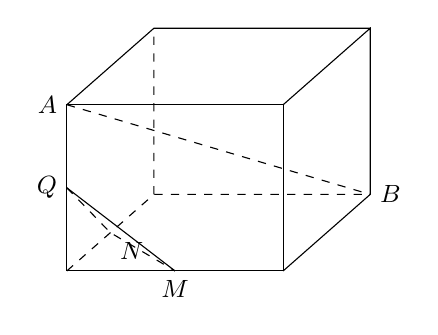
\begin{tikzpicture}[scale=.67, every node/.style={font=\small}]
  \coordinate (FBL) at (0,0);
  \coordinate (FBR) at (4.1,0);
  \coordinate (FTR) at (4.1,3.15);
  \coordinate (FTL) at (0,3.15);
  \coordinate (BBL) at (1.65,1.45);
  \coordinate (BBR) at (5.75,1.45);
  \coordinate (BTR) at (5.75,4.60);
  \coordinate (BTL) at (1.65,4.60);
  \coordinate (M) at (2.05,0);
  \coordinate (Q) at (0,1.575);
  \coordinate (N) at (.825,.725);

  \draw (FBL)--(FBR)--(FTR)--(FTL)--cycle;
  \draw (FTR)--(BTR)--(BBR)--(FBR);
  \draw (FTL)--(BTL)--(BTR);
  \draw[dashed] (FBL)--(BBL)--(BBR) (BBL)--(BTL);
  \draw[dashed] (FTL)--(BBR) (Q)--(N)--(M);
  \draw (Q)--(M);

  \node[left]        at (FTL) {$A$};
  \node[right]       at (BBR) {$B$};
  \node[below]       at (M)   {$M$};
  \node[left]        at (Q)   {$Q$};
  \node[below right] at (N)   {$N$};
\end{tikzpicture}
}}
    \task \raisebox{-.5\height}{\resizebox{0.13\textwidth}{!}{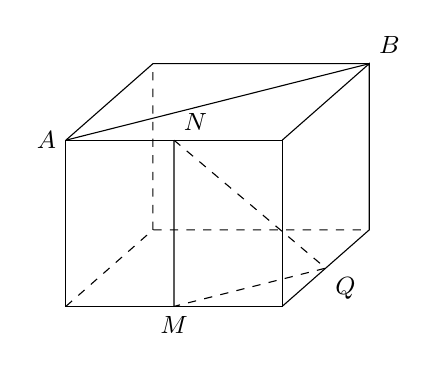
\begin{tikzpicture}[scale=.67, every node/.style={font=\small}]
  \coordinate (FBL) at (0,0);
  \coordinate (FBR) at (4.1,0);
  \coordinate (FTR) at (4.1,3.15);
  \coordinate (FTL) at (0,3.15);
  \coordinate (BBL) at (1.65,1.45);
  \coordinate (BBR) at (5.75,1.45);
  \coordinate (BTR) at (5.75,4.60);
  \coordinate (BTL) at (1.65,4.60);
  \coordinate (M) at (2.05,0);
  \coordinate (N) at (2.05,3.15);
  \coordinate (Q) at (4.925,.725);

  \draw (FBL)--(FBR)--(FTR)--(FTL)--cycle;
  \draw (FTR)--(BTR)--(BBR)--(FBR);
  \draw (FTL)--(BTL)--(BTR);
  \draw[dashed] (FBL)--(BBL)--(BBR) (BBL)--(BTL);
  \draw (FTL)--(BTR) (M)--(N);
  \draw[dashed] (N)--(Q)--(M);

  \node[left]        at (FTL) {$A$};
  \node[above right] at (BTR) {$B$};
  \node[below]       at (M)   {$M$};
  \node[above right] at (N)   {$N$};
  \node[below right] at (Q)   {$Q$};
\end{tikzpicture}
}}
    \task \raisebox{-.5\height}{\resizebox{0.13\textwidth}{!}{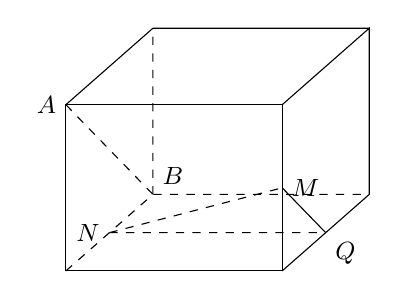
\begin{tikzpicture}[scale=.67, every node/.style={font=\small}]
  \coordinate (FBL) at (0,0);
  \coordinate (FBR) at (4.1,0);
  \coordinate (FTR) at (4.1,3.15);
  \coordinate (FTL) at (0,3.15);
  \coordinate (BBL) at (1.65,1.45);
  \coordinate (BBR) at (5.75,1.45);
  \coordinate (BTR) at (5.75,4.60);
  \coordinate (BTL) at (1.65,4.60);
  \coordinate (M) at (4.1,1.575);
  \coordinate (N) at (.825,.725);
  \coordinate (Q) at (4.925,.725);

  \draw (FBL)--(FBR)--(FTR)--(FTL)--cycle;
  \draw (FTR)--(BTR)--(BBR)--(FBR);
  \draw (FTL)--(BTL)--(BTR);
  \draw[dashed] (FBL)--(BBL)--(BBR) (BBL)--(BTL);
  \draw[dashed] (FTL)--(BBL) (N)--(M) (N)--(Q);
  \draw (M)--(Q);

  \node[left]        at (FTL) {$A$};
  \node[above right] at (BBL) {$B$};
  \node[right]       at (M)   {$M$};
  \node[left]        at (N)   {$N$};
  \node[below right] at (Q)   {$Q$};
\end{tikzpicture}
}}
    \task \raisebox{-.5\height}{\resizebox{0.13\textwidth}{!}{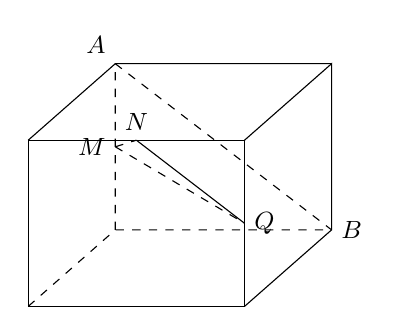
\begin{tikzpicture}[scale=.67, every node/.style={font=\small}]
  \coordinate (FBL) at (0,0);
  \coordinate (FBR) at (4.1,0);
  \coordinate (FTR) at (4.1,3.15);
  \coordinate (FTL) at (0,3.15);
  \coordinate (BBL) at (1.65,1.45);
  \coordinate (BBR) at (5.75,1.45);
  \coordinate (BTR) at (5.75,4.60);
  \coordinate (BTL) at (1.65,4.60);
  \coordinate (M) at (1.65,3.025);
  \coordinate (N) at (2.05,3.15);
  \coordinate (Q) at (4.1,1.575);

  \draw (FBL)--(FBR)--(FTR)--(FTL)--cycle;
  \draw (FTR)--(BTR)--(BBR)--(FBR);
  \draw (FTL)--(BTL)--(BTR);
  \draw[dashed] (FBL)--(BBL)--(BBR) (BBL)--(BTL);
  \draw[dashed] (BTL)--(BBR) (M)--(N) (M)--(Q);
  \draw (N)--(Q);

  \node[above left] at (BTL) {$A$};
  \node[right]      at (BBR) {$B$};
  \node[left]       at (M)   {$M$};
  \node[above]      at (N)   {$N$};
  \node[right]      at (Q)   {$Q$};
\end{tikzpicture}
}}
\end{tasks}
\end{example}
\begin{solution}
\textbf{答案：}A

A．因为直线 $AB$ 与平面 $MNQ$ 相交，所以直线 $AB$ 与平面 $MNQ$ 不平行

B．因为 $AB\px MQ$，且直线 $AB\not\subset$ 平面 $MNQ$，直线 $MQ\subset$ 平面 $MNQ$，所以直线 $AB\px$ 平面 $MNQ$

C．因为 $AB\px MQ$，且直线 $AB\not\subset$ 平面 $MNQ$，直线 $MQ\subset$ 平面 $MNQ$，所以直线 $AB\px$ 平面 $MNQ$

D．因为 $AB\px NQ$，且直线 $AB\not\subset$ 平面 $MNQ$，直线 $NQ\subset$ 平面 $MNQ$，所以直线 $AB\px$ 平面 $MNQ$

故选：A．
\end{solution}

\vspace{2em}

\begin{example}[\bkstar{3}{5}]
如图，在三棱柱 $ABC-A_1B_1C_1$ 中，$AM=2MA_1$，$BN=2NB_1$，过 $MN$ 作一平面交底面三角形 $ABC$ 的边 $BC$，$AC$ 于点 $E$，$F$（$E$、$F$ 与端点不重合），则
\bkfig{TikZ-final/geometry/solid/p014-o0307.tex}
\begin{tasks}(1)
    \task $MF\px NE$
    \task 四边形 $MNEF$ 为梯形
    \task 四边形 $MNEF$ 为平行四边形
    \task $A_1B_1\px NE$
\end{tasks}
\end{example}
\begin{solution}
\textbf{答案：}B

$\because$ 在平行四边形 $AA_1B_1B$ 中，$AM=2MA_1$，$BN=2NB_1$

$\therefore AM\overset{\px}{=}BN$

$\therefore MN\overset{\px}{=}AB$

又 $MN\not\subset$ 平面 $ABC$，$AB\subset$ 平面 $ABC$

$\therefore MN\px$ 平面 $ABC$

又 $MN\subset$ 平面 $MNEF$，平面 $MNEF\cap$ 平面 $ABC=EF$

$\therefore MN\px EF$

$\therefore EF\px AB$，显然在 $\triangle ABC$ 中，$EF\neq AB$

$\therefore EF\neq MN$

所以四边形 $MNEF$ 为梯形

故选：B．
\end{solution}

\vspace{2em}

\begin{example}[\bkstar{2}{5}]
如图，四棱锥 $P-ABCD$ 中，$M$，$N$ 分别为 $AC$，$PC$ 上的点，且 $MN\px$ 平面 $PAD$，则
\bkfig{TikZ-final/geometry/solid/p014-o0309.tex}
\begin{tasks}(1)
    \task $MN\px PD$
    \task $MN\px PA$
    \task $MN\px AD$
    \task 以上均有可能
\end{tasks}
\end{example}
\begin{solution}
\textbf{答案：}B

$\because MN\px$ 平面 $PAD$，$MN\subset$ 平面 $PAC$，平面 $PAC\cap$ 平面 $PAD=PA$，

$\therefore MN\px PA$．

故选：B．
\end{solution}

\vspace{2em}

\begin{example}[\bkstar{3}{5}]
在如图所示的正四棱柱 $ABCD-A_1B_1C_1D_1$ 中，$E$，$F$ 分别是棱 $B_1B$，$AD$ 的中点，直线 $BF$ 与平面 $AD_1E$ 的位置关系是
\bkfig{TikZ-final/geometry/solid/p014-o0311.tex}
\begin{tasks}(1)
    \task 平行
    \task 相交但不垂直
    \task 垂直
    \task 无法确定
\end{tasks}
\end{example}
\begin{solution}
\textbf{答案：}A

取 $AD_1$ 的中点 $O$，连接 $OE$，$OF$，则易得 $OF$ 平行且等于 $BE$
\bkfig{TikZ-final/geometry/solid/p058-o1189.tex}
$\therefore$ 四边形 $BFOE$ 是平行四边形

$\therefore BF\px OE$

$\because BF\not\subset$ 平面 $AD_1E$，$OE\subset$ 平面 $AD_1E$

$\therefore BF\px$ 平面 $AD_1E$

故选：A．
\end{solution}

\vspace{2em}

\begin{example}[\bkstar{3}{5}]
如图，在四棱锥 $P-ABCD$ 中，底面 $ABCD$ 是边长为 $a$ 的正方形，侧面 $PAD\perp$ 底面 $ABCD$，且 $PA=PD=\dfrac{\sqrt{2}}{2}AD$，设 $E$，$F$ 分别为 $PC$，$BD$ 的中点．求证：$EF\px$ 平面 $PAD$．
\bkfig[0.3\textwidth]{TikZ-final/geometry/solid/p015-o0324.tex}
\end{example}
\begin{solution}
\bkfig[0.3\textwidth]{TikZ-final/geometry/solid/p058-o1194.tex}
因为 $ABCD$ 为正方形，连接 $AC$ 交 $BD$ 于点 $F$

又因为在 $\triangle CPA$ 中，$F$ 为 $AC$ 中点，$E$ 为 $PC$ 中点

所以 $EF\px PA$，且 $PA\subset$ 平面 $PAD$，$EF\not\subset$ 平面 $PAD$ % 待核对：原书解析在此处截断，缺少结论句
\end{solution}

\vspace{2em}

\bktopic{平面与平面平行}

\begin{example}[\bkstar{3}{5}]
已知直四棱柱 $ABCD-A_1B_1C_1D_1$，$AD=DD_1=2$，$BC=DC=1$，$DC\perp BC$，$AD\px BC$，$E$，$F$ 分别为 $CC_1$，$DD_1$ 的中点．求证：面 $BEF\px$ 面 $AD_1C_1$．
\bkfig{TikZ-final/geometry/solid/p015-o0325.tex}
\end{example}
\begin{solution}
取 $AD$ 的中点 $G$，连接 $FG$，$BG$，如图所示
\bkfig{TikZ-final/geometry/solid/p059-o1207.tex}
$\because G$ 为 $AD$ 的中点，$AD=2$

$\therefore DG=1$

又 $AD\px BC$，$BC=1$

$\therefore DG\px BC$，$DG=BC$

$\therefore$ 四边形 $BCDG$ 为平行四边形

$\therefore BG\px CD$，$BG=CD$

又 $E$，$F$ 分别为 $CC_1$，$DD_1$ 的中点

$\therefore EF\px CD$，$EF=CD$

$\therefore BG\px EF$，$BG=EF$

$\therefore$ 四边形 $BEFG$ 为平行四边形

$\therefore GF\px BE$

又在 $\triangle ADD_1$ 中，$GF$ 为其中位线

$\therefore GF\px AD_1$

$\therefore AD_1\px BE$

又 $AD_1\not\subset$ 平面 $BEF$，$BE\subset$ 平面 $BEF$

$\therefore AD_1\px$ 平面 $BEF$

由 $E$，$F$ 分别为 $CC_1$，$DD_1$ 的中点，显然有 $C_1D_1\px EF$

又 $C_1D_1\not\subset$ 平面 $BEF$，$EF\subset$ 平面 $BEF$

$\therefore C_1D_1\px$ 平面 $BEF$

$\because AD_1\cap C_1D_1=D_1$

$\therefore$ 面 $BEF\px$ 面 $AD_1C_1$
\end{solution}

\vspace{2em}

\begin{example}[\bkstar{3}{5}]
已知平面 $\alpha\px$ 平面 $\beta$，$P$ 是 $\alpha$，$\beta$ 外一点，过 $P$ 点的两条直线 $PAC$，$PBD$ 分别交 $\alpha$ 于 $A$，$B$，交 $\beta$ 于 $C$，$D$，且 $PA=6$，$AC=9$，$AB=8$，则 $CD$ 的长为
\end{example}
\begin{solution}
\textbf{答案：}$20$ 或 $4$

如图所示，
\bkfig[0.45\textwidth]{TikZ-final/geometry/solid/p059-o1208.tex}
因为平面 $\alpha\px$ 平面 $\beta$

所以 $AB\px CD$

$\therefore \triangle PAB\backsim\triangle PCD$

$\therefore \dfrac{PA}{PC}=\dfrac{AB}{CD}$

$\therefore CD=\dfrac{8\times 15}{6}=20$

当 $P$ 在平面 $\alpha$ 与平面 $\beta$ 之间时

$\therefore \dfrac{PA}{PC}=\dfrac{AB}{CD}$

$\therefore CD=\dfrac{8\times 3}{6}=4$

故答案为：$20$ 或 $4$．
\end{solution}

\vspace{2em}

\bktopic{点共线、线共点问题}

\begin{example}[\bkstar{3}{5}]
如图，三棱锥 $P-ABC$ 中，$M$，$N$ 分别是 $AP$，$AB$ 的中点，$E$，$F$ 分别是 $PC$，$BC$ 上的点且 $\dfrac{PE}{EC}=\dfrac{BF}{FC}=2$，下列命题正确的是
\bkfig{TikZ-final/geometry/solid/p016-o0338.tex}
\begin{tasks}(1)
    \task $MN=EF$
    \task $ME$ 与 $NF$ 是异面直线
    \task $AC\px$ 平面 $MNFE$
    \task 直线 $ME$，$NF$，$AC$ 相交于同一点
\end{tasks}
\end{example}
\begin{solution}
\textbf{答案：}D

依题意，$M$，$N$ 分别是 $AP$，$AB$ 的中点，$E$，$F$ 分别是 $PC$，$BC$ 上的点且 $\dfrac{PE}{EC}=\dfrac{BF}{FC}=2$

所以 $MN\px PB$，$MN=\dfrac{1}{2}PB$，$EF\px PB$，$EF=\dfrac{1}{3}PB$

故A选项错误，B选项错误

易知 $M$，$E\in$ 平面 $APC$，$N$，$F\in$ 平面 $ABC$，平面 $APC\cap$ 平面 $ABC=AC$

设 $ME\cap NF=G$

则由公理 $3$ 知 $G\in AC$

即直线 $ME$，$NF$，$AC$ 相交于同一点 $G$

故D选项正确，C选项错误

故选：D．
\end{solution}

\vspace{2em}

\bktopic{点、线共面}

\begin{example}[\bkstar{2}{5}]
下列四个图形中，正方体棱上的四个中点共面的图形是
\bkfig[0.6\textwidth]{TikZ-final/geometry/solid/p016-o0339.tex}
\begin{tasks}(4)
    \task 甲与乙
    \task 乙与丙
    \task 丙与丁
    \task 丁与甲
\end{tasks}
\end{example}
\begin{solution}
\textbf{答案：}A

分别连接各中点，如图所示
\bkfig[0.6\textwidth]{TikZ-final/geometry/solid/p060-o1221.tex}
观察四个图形，则可发现正方体棱上的四个中点共面的图形是甲与乙

故选：A．
\end{solution}

\vspace{2em}

\subsection{提能力}
\bktopic{点、线确定平面问题}

\begin{example}[\bkstar{3}{5}]
在正方体 $ABCD-A_1B_1C_1D_1$ 中，$E$，$F$ 分别为棱 $AA_1$，$CC_1$ 的中点，则在空间中与三条直线 $A_1D_1$，$EF$，$CD$ 都相交的直线
\begin{tasks}(4)
    \task 不存在
    \task 有且只有两条
    \task 有且只有三条
    \task 有无数条
\end{tasks}
\end{example}
\begin{solution}
\textbf{答案：}D

\bkfig{TikZ-final/geometry/solid/p061-o1234.tex}
在 $EF$ 上任意取一点 $M$

直线 $A_1D_1$ 与 $M$ 确定一个平面

这个平面与 $CD$ 有且仅有 $1$ 个交点 $N$，当 $M$ 取不同的位置就确定不同的平面

从而与 $CD$ 有不同的交点 $N$

而直线 $MN$ 与这 $3$ 条异面直线都有交点．如图

故选：D．
\end{solution}

\vspace{2em}

\begin{example}[\bkstar{3}{5}]
在棱长为 $10$ 的正方体 $ABCD-A_1B_1C_1D_1$ 中，$P$ 为左侧面 $ADD_1A_1$ 上一点，已知点 $P$ 到 $A_1D_1$ 的距离为 $3$，$P$ 到 $AA_1$ 的距离为 $2$，则过点 $P$ 且与 $A_1C$ 平行的直线交正方体于 $P$，$Q$ 两点，则 $Q$ 点所在的平面是
\bkfig{TikZ-final/geometry/solid/p017-o0353.tex}
\begin{tasks}(4)
    \task $ABCD$
    \task $BB_1C_1C$
    \task $CC_1D_1D$
    \task $AA_1B_1B$
\end{tasks}
\end{example}
\begin{solution}
\textbf{答案：}A

如图，设直线 $A_1P$ 与线段 $AD$ 交于点 $E$，连接 $CE$
\bkfig{TikZ-final/geometry/solid/p061-o1236.tex}
可知过点 $P$ 且与 $A_1C$ 平行的直线在平面 $A_1EC$ 内，可知平面 $A_1EC$ 与平面 $ABCD$ 相交于直线 $CE$，点 $Q$ 在直线 $CE$ 上，也在平面 $ABCD$ 内

故选：A．
\end{solution}

\vspace{2em}

\bktopic{直线与平面平行}

\begin{example}[\bkstar{3}{5}]
如图，在各棱长均为 $a$ 的正三棱柱 $ABC-A_1B_1C_1$ 中，$M$，$N$ 分别为线段 $A_1B$，$B_1C$ 上的动点，且 $MN\px$ 平面 $ACC_1A_1$，则这样的 $MN$ 有
\bkfig{TikZ-final/geometry/solid/p017-o0355.tex}
\begin{tasks}(1)
    \task $1$ 条
    \task $2$ 条
    \task $3$ 条
    \task 无数条
\end{tasks}
\end{example}
\begin{solution}
\textbf{答案：}D

由题意得 $A_1B=CB_1=\sqrt{2}a$，在 $BA_1$，$CB_1$ 上分别取 $M$，$N$ 使 $BM=CN$，过 $M$，$N$ 分别作 $MM_1\perp AB$，$NN_1\perp BC$，垂足分别为 $M_1$，$N_1$
\bkfig{TikZ-final/geometry/solid/p061-o1238.tex}
则 $MM_1\px AA_1$，$NN_1\px BB_1$

故 $MM_1\px NN_1$，$\dfrac{BM}{BA_1}=\dfrac{MM_1}{AA_1}$，$\dfrac{CN}{B_1C}=\dfrac{NN_1}{BB_1}$

$\because \dfrac{BM}{BA_1}=\dfrac{CN}{B_1C}$

$\therefore \dfrac{MM_1}{AA_1}=\dfrac{NN_1}{BB_1}$

又 $\because AA_1=BB_1$

$\therefore MM_1=NN_1$，$MM_1\px NN_1$

$\therefore$ 四边形 $MNN_1M_1$ 是平行四边形

$\therefore MN\px M_1N_1$

可得 $M_1N_1\px$ 平面 $ACC_1A_1$

又 $\because MM_1\px$ 平面 $ACC_1A_1$，$M_1N_1\cap MM_1=M_1$

$\therefore$ 平面 $MM_1N_1N\px$ 平面 $ACC_1A_1$，由于 $MN\subset$ 平面 $MM_1N_1N$

所以 $MN\px$ 平面 $ACC_1A_1$，点 $M$，$N$ 是符合 $BM=CN$ 的动点，从而满足条件的 $MN$ 有无数条

故选：D．
\end{solution}

\vspace{2em}

\bktopic{平面与平面平行}

\begin{example}[\bkstar{3}{5}]
如图是正方体的平面展开图，在这个正方体中．
\bkfig[0.35\textwidth]{TikZ-final/geometry/solid/p017-o0356.tex}
\begin{enumerate}
    \item[\ding{172}] $BM\px$ 平面 $DE$
    \item[\ding{173}] $CN\px$ 平面 $AF$
    \item[\ding{174}] 平面 $BDM\px$ 平面 $AFN$
    \item[\ding{175}] 平面 $BDE\px$ 平面 $NCF$
\end{enumerate}
其中正确命题的序号是
\end{example}
\begin{solution}
\textbf{答案：}\ding{172}\ding{173}\ding{174}\ding{175}

把正方体的平面展开图还原成正方体 $ABCD-EFMN$
\bkfig{TikZ-final/geometry/solid/p062-o1252.tex}
\ding{172}$\because BM\px AN$，$BM\not\subset$ 平面 $DE$，$AN\subset$ 平面 $DE$

$\therefore BM\px$ 平面 $DE$，故正确

\ding{173}$\because CN\px BE$，$CN\not\subset$ 平面 $AF$，$BE\subset$ 平面 $AF$

$\therefore CN\px$ 平面 $AF$，故正确

\ding{174}$\because BD\px FN$，$BM\px AN$，$BD\cap BM=B$，$BD$，$BM\subset$ 平面 $BDM$

$FN\cap AN=N$，$FN$，$AN\subset$ 平面 $AFN$

$\therefore$ 平面 $BDM\px$ 平面 $AFN$，故正确

\ding{175}$\because BD\px FN$，$BE\px CN$，$BD\cap BE=B$，$BD$，$BE\subset$ 平面 $BDE$

$FN\cap CN=N$，$FN$，$CN\subset$ 平面 $NCF$

$\therefore$ 平面 $BDE\px$ 平面 $NCF$，故正确

故答案为：\ding{172}\ding{173}\ding{174}\ding{175}．
\end{solution}

\vspace{2em}

\begin{example}[\bkstar{3}{5}]
已知 $E$，$F$，$H$，$G$ 分别是四面体 $ABCD$ 棱 $AB$，$BC$，$CD$，$DA$ 上的点，且 $AE=EB$，$BF=FC$，$CH=2HD$，$AG=2GD$，则下列说法错误的是
\begin{tasks}(2)
    \task $AC\px$ 平面 $EFH$
    \task $BD\px$ 平面 $EFG$
    \task 直线 $EG$，$FH$，$BD$ 相交于同一点
    \task $FE\px GH$
\end{tasks}
\end{example}
\begin{solution}
\textbf{答案：}B

A．$EA=EB$，$BF=FC$，$CH=2HD$，$AG=2GD$，可得到 $GH\px AC$，$EF\px AC$，故得到 $AC\px$ 平面 $EFH$，选项正确

B．因为 $BD$ 和 $FH$ 不平行，而且两条直线在同一平面内，故得到两直线延长后相交，又 $BD\not\subset$ 平面 $EFG$，可得到 $BD$ 与平面 $EFG$ 是相交关系，选项不正确

C．由A选项，结合平行线的传递性得到 $GH\px EF$，则 $EFGH$ 四点共面，且为等腰梯形，延长 $EH$ 和 $FH$ 相交于点 $M$ 则点 $M$ 在 $FH$ 的延长线上，故在平面 $BDC$ 内，同理 $M$ 点也在平面 $ABD$ 内，故 $M$ 应该在两个平面的交线上，即直线 $BD$ 的延长线上，故得证，选项正确

D．$EA=EB$，$BF=FC$，$CH=2HD$，$AG=2GD$，可得到 $GH\px AC$，$EF\px AC$，由平行线的传递性得到 $FE\px GH$，选项正确

故选：B．
\end{solution}

\vspace{2em}

\begin{example}[\bkstar{3}{5}]
如图，在正方体 $ABCD-A_1B_1C_1D_1$ 中，$O$ 为底面 $ABCD$ 的中心，$P$ 是 $DD_1$ 的中点，设 $Q$ 是 $CC_1$ 上的点，当点 $Q$ 在（\quad）位置时，平面 $D_1BQ\px$ 平面 $PAO$．
\bkfig{TikZ-final/geometry/solid/p018-o0369.tex}
\begin{tasks}(1)
    \task $Q$ 与 $C$ 重合
    \task $Q$ 与 $C_1$ 重合
    \task $Q$ 为 $CC_1$ 的三等分点
    \task $Q$ 为 $CC_1$ 的中点
\end{tasks}
\end{example}
\begin{solution}
\textbf{答案：}D

在正方体 $ABCD-A_1B_1C_1D_1$

$\because O$ 为底面 $ABCD$ 的中心，$P$ 是 $DD_1$ 的中点

$\therefore PO\px BD_1$

设 $Q$ 是 $CC_1$ 上的点，当点 $Q$ 在 $CC_1$ 的中点位置时

$PQ\px AB$

$\therefore$ 四边形 $ABQP$ 是平行四边形

$\therefore AP\px BQ$

$\because AP\cap PO=P$，$BQ\cap BD_1=B$，$AP$，$PO\subset$ 平面 $APO$，$BQ$，$BD_1\subset$ 平面 $BQD_1$

$\therefore$ 平面 $D_1BQ\px$ 平面 $PAO$

故选：D．
\end{solution}

\vspace{2em}

\section{第3讲\quad 空间中的垂直关系}
\subsection{夯基础}
\bktopic{直线与平面垂直}

\begin{example}[\bkstar{1}{5}]
垂直于同一平面的两条直线一定
\begin{tasks}(4)
    \task 平行
    \task 相交
    \task 异面
    \task 以上都有可能
\end{tasks}
\end{example}
\begin{solution}
\textbf{答案：}A

设直线 $a$、$b$ 都与平面 $\alpha$ 垂直，可以用反证法证明 $a$、$b$ 必定是平行直线．假设 $a$、$b$ 不平行，过直线 $b$ 与平面 $\alpha$ 的交点作直线 $d$，使 $d\px a$，$\therefore$ 直线 $d$ 与直线 $b$ 是相交直线，设它们确定平面 $\beta$，且 $\beta\cap\alpha=c$．$\because b\perp\alpha$，$c\subset\alpha$，$\therefore b\perp c$．同理可得 $a\perp c$，又 $\because d\px a$，$\therefore d\perp c$．这样经过一点作出两条直线 $b$、$d$ 都与直线 $c$ 垂直，这是不可能的，$\therefore$ 假设不成立，故原命题是真命题．

故选：A．
\end{solution}

\vspace{2em}

\begin{example}[\bkstar{1}{5}]
一条直线与一个平面垂直的条件是这条直线
\begin{tasks}(2)
    \task 垂直于平面内的一条直线
    \task 垂直于平面内的两条直线
    \task 垂直于平面内的无数条直线
    \task 垂直于平面内的两条相交直线
\end{tasks}
\end{example}
\begin{solution}
\textbf{答案：}D

由线面垂直的判定定理，可得一条直线与一个平面垂直的条件是这条直线垂直于平面内的两条相交直线．

故选：D．
\end{solution}

\vspace{2em}

\begin{example}[\bkstar{2}{5}]
已知直线 $m$ 和平面 $\alpha$，$\beta$，若 $\alpha\perp\beta$，$m\perp\alpha$，则
\begin{tasks}(4)
    \task $m\perp\beta$
    \task $m\px\beta$
    \task $m\subset\beta$
    \task $m\px\beta$ 或 $m\subset\beta$
\end{tasks}
\end{example}
\begin{solution}
\textbf{答案：}D

结合线面垂直和面面垂直可知答案为 D．

故选：D．
\end{solution}

\vspace{2em}

\begin{example}[\bkstar{2}{5}]
正方体 $ABCD-A_1B_1C_1D_1$ 中，与 $AD_1$ 垂直的平面是
\begin{tasks}(4)
    \task 平面 $DD_1C_1C$
    \task 平面 $A_1DB$
    \task 平面 $A_1B_1C_1D_1$
    \task 平面 $A_1DB_1$
\end{tasks}
\end{example}
\begin{solution}
\textbf{答案：}D

正方体 $ABCD-A_1B_1C_1D_1$ 中，

在 A 中，$AD_1$ 与平面 $DD_1C_1C$ 相交但不垂直，故 A 错误；

在 B 中，$AD_1$ 与平面 $A_1DB$ 相交但不垂直，故 B 错误；

在 C 中，$AD_1$ 与平面 $A_1B_1C_1D_1$ 相交但不垂直，故 C 错误；

在 D 中，$AD_1\perp A_1D$，$AD_1\perp A_1B_1$，$A_1D\cap A_1B_1=A_1$，$\therefore AD_1\perp$ 平面 $A_1DB_1$，故 D 正确．

故选：D．
\end{solution}

\vspace{2em}

\begin{example}[\bkstar{2}{5}]
如图，四个正方体中，直线 $AB$ 与平面 $CDE$ 垂直的是
\bkfig[0.8\textwidth]{TikZ-final/geometry/solid/p020-o0431.tex}
\begin{tasks}(4)
    \task ①②
    \task ②④
    \task ①③
    \task ②③
\end{tasks}
\end{example}
\begin{solution}
\textbf{答案：}B

在题图①中，$AB$ 与 $CE$ 所成的角为 $45^{\circ}$，$\therefore$ 直线 $AB$ 与平面 $CDE$ 不垂直，故错误；

在题图②中，$AB\perp EC$，$AB\perp ED$，$EC\cap ED=E$，$\therefore AB\perp$ 平面 $CDE$，故正确；

在题图③中，$AB$ 与 $EC$ 所成的角为 $60^{\circ}$，$\therefore$ 直线 $AB$ 与平面 $CDE$ 不垂直，故错误；

在题图④中，$AB\perp DE$，$AB\perp CE$，$EC\cap ED=E$，$\therefore AB\perp$ 平面 $CDE$，故正确．

故选：B．
\end{solution}

\vspace{2em}

\begin{example}[\bkstar{2}{5}]
如图，在棱长为 $1$ 的正方体 $ABCD-A_1B_1C_1D_1$ 中．求证：$AC\perp$ 平面 $B_1BDD_1$．
\bkfig{TikZ-final/geometry/solid/p020-o0433.tex}
\end{example}
\begin{solution}
$\because$ 几何体 $ABCD-A_1B_1C_1D_1$ 是正方体，$\therefore$ 四边形 $ABCD$ 是正方形，$\therefore AC\perp BD$．又 $BB_1\perp$ 平面 $ABCD$，而 $AC\subset$ 平面 $ABCD$，$\therefore BB_1\perp AC$．

$$
\because \begin{cases} AC\perp BD \\ AC\perp BB_1 \end{cases}\text{，$BD$，$BB_1$ 是平面 $B_1BDD_1$ 内的两条相交直线}
$$

$\therefore AC\perp$ 平面 $B_1BDD_1$．
\end{solution}

\vspace{2em}

\begin{example}[\bkstar{2}{5}]
如图，在三棱锥 $P-ABC$ 中，$PA$ 垂直于平面 $ABC$，$AC\perp BC$，求证：$BC\perp$ 平面 $PAC$．
\bkfig{TikZ-final/geometry/solid/p020-o0434.tex}
\end{example}
\begin{solution}
$\because PA\perp$ 平面 $ABC$，$BC$ 在平面 $ABC$ 内，$\therefore PA\perp BC$．又 $\because AC\perp BC$，$PA\cap AC=A$，$\therefore BC\perp$ 平面 $PAC$．
\end{solution}

\vspace{2em}

\bktopic{平面与平面垂直判定}

\begin{example}[\bkstar{2}{5}]
如图，在立体图形 $D-ABC$ 中，若 $AB=CB$，$AD=CD$，$E$ 是 $AC$ 的中点，则下列结论正确的是
\bkfig{TikZ-final/geometry/solid/p020-o0436.tex}
\begin{tasks}(1)
    \task 平面 $ABC\perp$ 平面 $ABD$
    \task 平面 $ABD\perp$ 平面 $BDC$
    \task 平面 $ABC\perp$ 平面 $BDE$，且平面 $ADC\perp$ 平面 $BDE$
    \task 平面 $ABC\perp$ 平面 $ADC$，且平面 $ADC\perp$ 平面 $BDE$
\end{tasks}
\end{example}
\begin{solution}
\textbf{答案：}C

因为 $AB=CB$，且 $E$ 是 $AC$ 的中点，所以 $BE\perp AC$．同理有 $DE\perp AC$，且 $BE\cap DE=E$，于是 $AC\perp$ 平面 $BDE$．因为 $AC\subset$ 平面 $ABC$ 内，所以平面 $ABC\perp$ 平面 $BDE$．又因为 $AC\subset$ 平面 $ACD$，所以平面 $ACD\perp$ 平面 $BDE$．

故选：C．
\end{solution}

\vspace{2em}

\bktopic{直线与直线垂直}

\begin{example}[\bkstar{2}{5}]
如图，$PA\perp$ 矩形 $ABCD$，下列结论中不正确的是
\bkfig[0.35\textwidth]{TikZ-final/geometry/solid/p021-o0449.tex}
\begin{tasks}(4)
    \task $PD\perp BD$
    \task $PD\perp CD$
    \task $PB\perp BC$
    \task $PA\perp BD$
\end{tasks}
\end{example}
\begin{solution}
\textbf{答案：}A

$\because PA\perp$ 矩形 $ABCD$，$\therefore PA\perp CD$，又 $AD\perp CD$，$PA\cap AD=A$，$\therefore CD\perp$ 平面 $PAD$，$\therefore PD\perp CD$，故 B 正确．

又由 $AB\px CD$，则 $BA\perp$ 平面 $PAD$．$\because PA\perp$ 矩形 $ABCD$，$\therefore PA\perp BD$，若 $PD\perp BD$，由于 $PA\cap PD=P$，则 $BD\perp$ 平面 $PAD$，又 $BA\perp$ 平面 $PAD$，则过平面外一点有两条直线与平面垂直，不成立，故 $PD\perp BD$ 不正确，故 A 不正确．

$\because PA\perp$ 矩形 $ABCD$，$\therefore$ 由三垂线定理得 $PB\perp BC$，故 C 正确．

$\because PA\perp$ 矩形 $ABCD$，$\therefore$ 由直线与平面垂直的性质得 $PA\perp BD$，故 D 正确．

故选：A．
\end{solution}

\vspace{2em}

\begin{example}[\bkstar{2}{5}]
如图，$O$ 为正方体 $ABCD-A_1B_1C_1D_1$ 的底面 $ABCD$ 的中心，则下列直线中与 $B_1O$ 垂直的是
\bkfig{TikZ-final/geometry/solid/p021-o0450.tex}
\begin{tasks}(4)
    \task $A_1D$
    \task $AA_1$
    \task $A_1D_1$
    \task $A_1C_1$
\end{tasks}
\end{example}
\begin{solution}
\textbf{答案：}D

连接 $B_1D_1$．$\because ABCD-A_1B_1C_1D_1$ 是正方体，$\therefore BB_1\perp$ 平面 $A_1B_1C_1D_1$．$\because A_1C_1\subset$ 平面 $A_1B_1C_1D_1$，$\therefore BB_1\perp A_1C_1$．$\because A_1B_1C_1D_1$ 是正方形，$\therefore B_1D_1\perp A_1C_1$．$\because B_1D_1$，$BB_1$ 是平面 $BB_1D_1D$ 内的相交直线，$\therefore A_1C_1\perp$ 平面 $BB_1D_1D$．$\because B_1O\subset$ 平面 $BB_1D_1D$，$\therefore A_1C_1\perp B_1O$．

故选：D．
\end{solution}

\vspace{2em}

\subsection{刷中档}
\bktopic{由点线面位置关系判定结论}

\begin{example}[\bkstar{2}{5}]
已知直线 $a$，$b$ 都不在平面 $\alpha$ 内，则下列命题错误的是
\begin{tasks}(2)
    \task 若 $a\px b$，$a\px\alpha$，则 $b\px\alpha$
    \task 若 $a\px b$，$a\perp\alpha$，则 $b\perp\alpha$
    \task 若 $a\perp b$，$a\px\alpha$，则 $b\perp\alpha$
    \task 若 $a\perp b$，$a\perp\alpha$，则 $b\px\alpha$
\end{tasks}
\end{example}
\begin{solution}
\textbf{答案：}C

当 $a\perp b$，$a\px\alpha$ 时，$b$ 与 $\alpha$ 的位置关系可以是平行或相交．

故选：C．
\end{solution}

\vspace{2em}

\begin{example}[\bkstar{2}{5}]
已知不同的两条直线 $m$，$n$，不同的两个平面 $\alpha$，$\beta$，给出下列命题：
\begin{enumerate}
    \item[①] 若 $m\perp\alpha$，$n\perp\beta$，且 $m\perp n$，则 $\alpha\perp\beta$
    \item[②] 若 $m\px\alpha$，$n\px\beta$，且 $m\px n$，则 $\alpha\px\beta$
    \item[③] 若 $m\perp\alpha$，$n\px\beta$，且 $m\perp n$，则 $\alpha\px\beta$
    \item[④] 若 $m\perp\alpha$，$n\px\beta$，且 $m\px n$，则 $\alpha\perp\beta$
\end{enumerate}
其中正确的命题是
\begin{tasks}(4)
    \task ②③
    \task ①③
    \task ①④
    \task ③④
\end{tasks}
\end{example}
\begin{solution}
\textbf{答案：}C

①若 $m\perp\alpha$，$n\perp\beta$，且 $m\perp n$，利用面面垂直的判定定理可得 $\alpha\perp\beta$，因此正确；

②若 $m\px\alpha$，$n\px\beta$，且 $m\px n$，则 $\alpha\px\beta$ 或相交，因此不正确；

③若 $m\perp\alpha$，$n\px\beta$，且 $m\perp n$，则 $\alpha\px\beta$ 或相交，因此不正确；

④若 $m\perp\alpha$，$n\px\beta$，且 $m\px n$，利用面面垂直的判定定理可得 $\alpha\perp\beta$，因此正确．

可知只有①④正确．

故选：C．
\end{solution}

\vspace{2em}

\begin{example}[\bkstar{2}{5}]
已知 $l$，$m$ 是平面 $\alpha$ 外的两条不同直线，给出下列三个论断：

①$l\perp m$；②$m\px\alpha$；③$l\perp\alpha$．

以其中的两个论断作为条件，余下的一个论断作为结论，写出一个正确的命题：
\end{example}
\begin{solution}
\textbf{答案：}若 $m\px\alpha$，$l\perp\alpha$，则 $l\perp m$．（答案不唯一）

当①②作为条件时，$l$ 与平面 $\alpha$ 的位置关系可能为平行或相交，故③不成立；当①③作为条件时，②成立；当②③作为条件时，①成立．
\end{solution}

\vspace{2em}

\bktopic{直线与平面垂直}

\begin{example}[\bkstar{2}{5}]
如果一条直线垂直于一个平面内的下列各种情况，能保证该直线与平面垂直的是
\begin{enumerate}
    \item[①] 三角形的两边
    \item[②] 梯形的两边
    \item[③] 圆的两条直径
    \item[④] 正六边形的两条边
\end{enumerate}
\begin{tasks}(4)
    \task ①③
    \task ②
    \task ②④
    \task ①②④
\end{tasks}
\end{example}
\begin{solution}
\textbf{答案：}A

因为三角形的任意两边是相交的，所以①可以证明线面垂直；因为梯形的上下两边是平行的，此时不相交，所以②不一定能保证线面垂直；因为圆的任意两条直径必相交，所以③可以证明线面垂直；因为正六边形的对边是平行的，所以④不一定能保证线面垂直．综上所述，正确的条件是：①③．

故选：A．
\end{solution}

\vspace{2em}

\begin{example}[\bkstar{3}{5}]
如图，在正三棱锥 $P-ABC$ 中，$E$，$F$，$G$ 分别为线段 $PA$，$PB$，$BC$ 的中点．求证：$BC\perp$ 平面 $PAG$．
\bkfig{TikZ-final/geometry/solid/p022-o0467.tex}
\end{example}
\begin{solution}
由正三棱锥可知，$\triangle ABC$，$\triangle PBC$ 均为等腰三角形．$\because G$ 为线段 $BC$ 的中点，$\therefore AG\perp BC$，$PG\perp BC$，且 $AG\cap PG=G$，$AG$，$PG\subset$ 平面 $PAG$，$\therefore BC\perp$ 平面 $PAG$．
\end{solution}

\vspace{2em}

\begin{example}[\bkstar{3}{5}]
如图，在三棱锥 $D-ABC$ 中，已知 $AC\perp BC$，$AC\perp DC$，$BC=DC$，$E$，$F$ 分别为 $BD$，$CD$ 的中点．求证：$BD\perp$ 平面 $ACE$．
\bkfig[0.35\textwidth]{TikZ-final/geometry/solid/p023-o0484.tex}
\end{example}
\begin{solution}
因为 $AC\perp BC$，$AC\perp DC$，$BC\cap DC=C$，所以 $AC\perp$ 平面 $BCD$．又 $BD\subset$ 平面 $BCD$，所以 $BD\perp AC$．又 $BC=DC$，$E$ 为 $BD$ 的中点，所以 $BD\perp CE$．又 $AC\cap CE=C$，所以 $BD\perp$ 平面 $ACE$．
\end{solution}

\vspace{2em}

\bktopic{直线与直线垂直}

\begin{example}[\bkstar{3}{5}]
如图，在 $\text{Rt}\triangle ABC$ 中，$\angle ABC=90^{\circ}$，$P$ 为 $\triangle ABC$ 所在平面外一点，$PA\perp$ 平面 $ABC$，则四面体 $P-ABC$ 中共有（\qquad）个直角三角形．
\bkfig{TikZ-final/geometry/solid/p023-o0485.tex}
\begin{tasks}(4)
    \task $4$
    \task $3$
    \task $2$
    \task $1$
\end{tasks}
\end{example}
\begin{solution}
\textbf{答案：}A

在 $\text{Rt}\triangle ABC$ 中，$\angle ABC=90^{\circ}$，$P$ 为 $\triangle ABC$ 所在平面外一点，$PA\perp$ 平面 $ABC$，$\therefore BC\perp PA$，$BC\perp AB$，$\because PA\cap AB=A$，$\therefore BC\perp$ 平面 $PAB$，$\therefore$ 四面体 $P-ABC$ 中直角三角形有 $\triangle PAC$，$\triangle PAB$，$\triangle ABC$，$\triangle PBC$．

故选：A．
\end{solution}

\vspace{2em}

\begin{example}[\bkstar{3}{5}]
如图，在 $\triangle ABC$ 中，$PA\perp$ 面 $ABC$，$AB=AC$，$D$ 是 $BC$ 的中点，则图中直角三角形的个数是
\bkfig{TikZ-final/geometry/solid/p023-o0486.tex}
\begin{tasks}(4)
    \task $5$
    \task $6$
    \task $7$
    \task $8$
\end{tasks}
\end{example}
\begin{solution}
\textbf{答案：}C

$\because$ 在 $\triangle ABC$ 中，$PA\perp$ 面 $ABC$，$AB=AC$，$D$ 是 $BC$ 的中点，$\therefore$ 图中直角三角形有 $\triangle ABD$，$\triangle ADC$，$\triangle PAD$，$\triangle PAB$，$\triangle PAC$，$\triangle PBD$，$\triangle PCD$，共 $7$ 个．

故选：C．
\end{solution}

\vspace{2em}

\bktopic{平面与平面垂直的性质}

\begin{example}[\bkstar{3}{5}]
已知平面 $\alpha$，$\beta$，$\gamma$ 两两垂直，直线 $a$，$b$，$c$ 满足：$a\subset\alpha$，$b\subset\beta$，$c\subset\gamma$，则直线 $a$，$b$，$c$ 不可能满足以下哪种关系
\begin{tasks}(4)
    \task 两两垂直
    \task 两两平行
    \task 两两相交
    \task 两两异面
\end{tasks}
\end{example}
\begin{solution}
\textbf{答案：}B

如图，可得 $a$，$b$，$c$ 可能两两垂直，且两两异面．
\bkfig[0.3\textwidth]{TikZ-final/geometry/solid/p070-o1385.tex}
如图，可得 $a$，$b$，$c$ 可能两两相交．
\bkfig[0.3\textwidth]{TikZ-final/geometry/solid/p070-o1386.tex}

故选：B．
\end{solution}

\vspace{2em}

\begin{example}[\bkstar{3}{5}]
下列命题中错误的是
\begin{tasks}(1)
    \task 如果平面 $\alpha\perp$ 平面 $\gamma$，平面 $\beta\perp$ 平面 $\gamma$，$\alpha\cap\beta=l$，那么 $l\perp\gamma$
    \task 如果平面 $\alpha\perp$ 平面 $\beta$，那么平面 $\alpha$ 内一定存在直线平行于平面 $\beta$
    \task 如果平面 $\alpha\perp$ 平面 $\beta$，过 $\alpha$ 与 $\beta$ 交线上的点作交线的垂线，那么此垂线必垂直于 $\beta$
    \task 如果平面 $\alpha$ 不垂直于平面 $\beta$，那么平面 $\alpha$ 内一定不存在直线垂直于平面 $\beta$
\end{tasks}
\end{example}
\begin{solution}
\textbf{答案：}C

A．平面 $\alpha\perp$ 平面 $\gamma$，平面 $\beta\perp$ 平面 $\gamma$，$\alpha\cap\beta=l$，则 $l\perp\gamma$，命题正确；

B．平面 $\alpha\perp$ 平面 $\beta$，不妨设 $\alpha\cap\beta=a$，作直线 $b\px a$，且 $b\subset\alpha$，则 $b\px\beta$，命题正确；

C．平面 $\alpha\perp$ 平面 $\beta$，过 $\alpha$ 与 $\beta$ 交线上的点作交线的垂线时，该垂线不一定垂直于 $\beta$，命题错误；

D．假设平面 $\alpha$ 内存在直线垂直于平面 $\beta$，则平面 $\alpha$ 垂直于平面 $\beta$，这与已知平面 $\alpha$ 与平面 $\beta$ 不垂直矛盾，所以假设不成立，命题正确．

故选：C．
\end{solution}

\vspace{2em}

\subsection{提能力}
\bktopic{平面与平面垂直的性质}

\begin{example}[\bkstar{3}{5}]
如图所示，在四面体 $P-ABC$ 中，$PB=\sqrt{13}$，平面 $PAB\perp$ 平面 $ABC$，$\angle ABC=90^{\circ}$，$BC=6$，则 $PC=$
\bkfig{TikZ-final/geometry/solid/p024-o0499.tex}
\begin{tasks}(4)
    \task $7$
    \task $8$
    \task $9$
    \task $10$
\end{tasks}
\end{example}
\begin{solution}
\textbf{答案：}A

因为平面 $PAB\perp$ 平面 $ABC$，$\angle ABC=90^{\circ}$，又因为 $BC\subset$ 平面 $ABC$，平面 $PAB\cap$ 平面 $ABC=AB$，所以 $BC\perp$ 平面 $PAB$．又因为 $PB\subset$ 平面 $PAB$，所以 $BC\perp PB$，则在直角三角形 $PBC$ 中，$PC=\sqrt{PB^2+BC^2}=\sqrt{13+36}=7$．

故选：A．
\end{solution}

\vspace{2em}

\begin{example}[\bkstar{3}{5}]
在四面体 $ABCD$ 中，$AB\perp AD$，$AB=AD=BC=CD=1$，且平面 $ABD\perp$ 平面 $BCD$，$M$ 为 $AB$ 的中点，则线段 $CM$ 的长为
\begin{tasks}(4)
    \task $\sqrt{2}$
    \task $\sqrt{3}$
    \task $\dfrac{\sqrt{3}}{2}$
    \task $\dfrac{\sqrt{2}}{2}$
\end{tasks}
\end{example}
\begin{solution}
\textbf{答案：}C
\bkfig[0.3\textwidth]{TikZ-final/geometry/solid/p071-o1399.tex}
因为 $AB\perp AD$，$AB=AD=1$，所以 $BD=\sqrt{2}$．又因为 $BC=CD=1$，所以 $BC\perp CD$．过点 $M$ 作 $MN\perp BD$ 交 $BD$ 于点 $N$，连结 $NC$，$MC$．因为平面 $ABD\perp$ 平面 $BCD$，平面 $ABD\cap$ 平面 $BCD=BD$，$MN\perp BD$，所以 $MN\perp$ 平面 $BCD$，所以 $MN\perp NC$．因为 $AB=AD=1$，$BC=CD=1$，$M$ 为 $AB$ 的中点，取 $BD$ 中点 $E$，连接 $CE$，在 $\text{Rt}\triangle ABD$ 和 $\text{Rt}\triangle CEN$ 中，计算得

$$
MN=\frac{\sqrt{2}}{4}\text{，}\quad CN=\sqrt{\left(\frac{\sqrt{2}}{2}\right)^2+\left(\frac{\sqrt{2}}{4}\right)^2}=\sqrt{\frac{5}{8}}\text{，}
$$

所以 $CM=\sqrt{MN^2+CN^2}=\dfrac{\sqrt{3}}{2}$．

故选：C．
\end{solution}

\vspace{2em}

\bktopic{平面与平面垂直的判定}

\begin{example}[\bkstar{3}{5}]
如图，以等腰直角三角形 $ABC$ 的斜边 $BC$ 上的高 $AD$ 为折痕，把 $\triangle ABD$ 和 $\triangle ACD$ 折成互相垂直的两个平面后，某学生得出下列四个结论．
\begin{enumerate}
    \item[①] $BD\perp AC$；
    \item[②] $\triangle BAC$ 是等边三角形；
    \item[③] 三棱锥 $D-ABC$ 是正三棱锥；
    \item[④] 平面 $ADC\perp$ 平面 $ABC$．
\end{enumerate}
其中正确的是
\bkfig[0.45\textwidth]{TikZ-final/geometry/solid/p025-o0512.tex}
\begin{tasks}(4)
    \task ①②④
    \task ①②③
    \task ②③④
    \task ①③④
\end{tasks}
\end{example}
\begin{solution}
\textbf{答案：}B

设 $\triangle ABC$ 的腰为 $a$，则斜边 $BC=\sqrt{2}a$．

①$\because D$ 为 $BC$ 的中点，$\therefore AD\perp BC$，又平面 $ABD\perp$ 平面 $ACD$，平面 $ABD\cap$ 平面 $ACD=AD$，$BD\perp AD$，$BD\subset$ 平面 $ABD$，$\therefore BD\perp$ 平面 $ADC$，又 $AC\subset$ 平面 $ADC$，$\therefore BD\perp AC$，故①正确；

②由①知，$BD\perp$ 平面 $ADC$，$CD\subset$ 平面 $ADC$，$\therefore BD\perp CD$，又 $BD=CD=\dfrac{\sqrt{2}}{2}a$，$\therefore$ 由勾股定理得 $BC=\sqrt{2}\cdot\dfrac{\sqrt{2}}{2}a=a$，又 $\because AB=AC=a$，$\therefore \triangle ABC$ 是等边三角形，故②正确；

③$\because \triangle ABC$ 是等边三角形，$DA=DB=DC$，$\therefore$ 三棱锥 $D-ABC$ 是正三棱锥，故③正确；

④$\because \triangle ADC$ 为等腰直角三角形，取斜边 $AC$ 的中点 $F$，则 $DF\perp AC$，又 $\triangle ABC$ 为等边三角形，连接 $BF$，则 $BF\perp AC$，$\therefore \angle BFD$ 为平面 $ADC$ 与平面 $ABC$ 的二面角的平面角，由 $BD\perp$ 平面 $ADC$ 可知，$\angle BDF$ 为直角，$\angle BFD$ 不是直角，故平面 $ADC$ 与平面 $ABC$ 不垂直，故④错误．

综上所述，正确的结论是①②③．

故选：B．
\end{solution}

\vspace{2em}

\bktopic{直线与直线的垂直}

\begin{example}[\bkstar{3}{5}]
如图所示，四边形 $ABCD$ 中，$AD\px BC$，$AD=AB$，$\angle BAD=\angle BDC=90^{\circ}$，将 $\triangle ABD$ 沿 $BD$ 折起，使平面 $ABD\perp$ 平面 $BCD$，构成三棱锥 $A-BCD$，则在三棱锥 $A-BCD$ 中，下列说法不正确的是
\bkfig[0.45\textwidth]{TikZ-final/geometry/solid/p025-o0513.tex}
\begin{tasks}(2)
    \task 直线 $BC\perp$ 直线 $AD$
    \task 直线 $CD\perp$ 直线 $AB$
    \task 直线 $CD\perp$ 平面 $ABD$
    \task 平面 $ACD\perp$ 平面 $ABD$
\end{tasks}
\end{example}
\begin{solution}
\textbf{答案：}A
\bkfig{TikZ-final/geometry/solid/p072-o1412.tex}
取 $BD$ 的中点 $E$．连接 $AE$，则 $AE\perp BD$．$\because$ 平面 $ABD\perp$ 平面 $BCD$，$AE\subset$ 平面 $BCD$，$\therefore AE\perp$ 平面 $BCD$，又 $BC\subset$ 平面 $BCD$，$\therefore AE\perp BC$，假设 $BC\perp AD$，因为 $AD$ 与 $AE$ 交于 $E$，$\therefore BC\perp$ 平面 $ABD$，又 $BD\subset$ 平面 $BCD$，$\therefore BC\perp BD$，这与 $\angle BDC=90^{\circ}$ 相矛盾，故假设不成立，即直线 $BC\perp$ 直线 $AD$ 不成立．% 待核对：原书两处写“平面 BCD”（AE⊂平面BCD、BD⊂平面BCD），按原书照录，疑应为平面 ABD

故选：A．
\end{solution}

\vspace{2em}

\begin{example}[\bkstar{4}{5}]
已知矩形 $ABCD$，$AB=1$，$BC=\sqrt{2}$，将 $\triangle ABD$ 沿矩形的对角线 $BD$ 所在的直线进行翻折，在翻折过程中
\begin{tasks}(1)
    \task 存在某个位置，使得直线 $AC$ 与直线 $BD$ 垂直
    \task 存在某个位置，使得直线 $AB$ 与直线 $CD$ 垂直
    \task 存在某个位置，使得直线 $AD$ 与直线 $BC$ 垂直
    \task 对任意位置，三对直线“$AC$ 与 $BD$”，“$AB$ 与 $CD$”，“$AD$ 与 $BC$”均不垂直
\end{tasks}
\end{example}
\begin{solution}
\textbf{答案：}B

作 $AE\perp BD$，$CF\perp BD$，依题意，$AB=1$，$BC=\sqrt{2}$，$AE=CF=\dfrac{\sqrt{6}}{3}$，$BE=EF=FD=\dfrac{\sqrt{3}}{3}$．

A．若存在某个位置，使得直线 $AC$ 与直线 $BD$ 垂直，则 $\because BD\perp AE$，$\therefore BD\perp$ 平面 $AEC$，从而 $BD\perp EC$，这与已知矛盾，排除 A；

B．若存在某个位置，使得直线 $AB$ 与直线 $CD$ 垂直，则 $CD\perp$ 平面 $ABC$，平面 $ABC\perp$ 平面 $BCD$．取 $BC$ 中点 $M$，连接 $ME$，则 $ME\perp BD$，$\therefore \angle AEM$ 就是二面角 $A-BD-C$ 的平面角，此角显然存在，即当 $A$ 在底面上的射影位于 $BC$ 的中点时，直线 $AB$ 与直线 $CD$ 垂直，故 B 正确；

C．若存在某个位置，使得直线 $AD$ 与直线 $BC$ 垂直，则 $BC\perp$ 平面 $ACD$，从而平面 $ACD\perp$ 平面 $BCD$，即 $A$ 在底面 $BCD$ 上的射影应位于线段 $CD$ 上，这是不可能的，排除 C；

D．由上所述，可排除 D．

故选：B．
\end{solution}

\vspace{2em}

\begin{example}[\bkstar{4}{5}]
如图，在直二面角 $A-BD-C$ 中，$\triangle ABD$，$\triangle CBD$ 均是以 $BD$ 为斜边的等腰直角三角形，取 $AD$ 的中点 $E$，将 $\triangle ABE$ 沿 $BE$ 翻折到 $\triangle A_1BE$，在翻折过程中，下列不可能成立的是
\bkfig[0.3\textwidth]{TikZ-final/geometry/solid/p026-o0526.tex}
\begin{tasks}(2)
    \task $BC$ 与平面 $A_1BE$ 内某直线平行
    \task $CD\px$ 平面 $A_1BE$
    \task $BC$ 与平面 $A_1BE$ 内某直线垂直
    \task $BC\perp A_1B$
\end{tasks}
\end{example}
\begin{solution}
\textbf{答案：}D
\bkfig[0.3\textwidth]{TikZ-final/geometry/solid/p073-o1425.tex}
连结 $CE$，当平面 $A_1BE$ 与平面 $BCE$ 重合时，$BC\subset$ 平面 $A_1BE$，$\therefore$ 平面 $A_1BE$ 内必存在与 $BC$ 平行和垂直的直线，故 A、C 可能成立．在平面 $BCD$ 内，过 $B$ 作 $CD$ 的平行线 $BF$，使得 $BF=CD$，连结 $EF$，$FC$，则当平面 $A_1BE$ 与平面 $BEF$ 重合时，$BF\subset$ 平面 $A_1BE$，故平面 $A_1BE$ 内存在与 $BF$ 平行的直线，即平面 $A_1BE$ 内存在与 $CD$ 平行的直线，$\therefore CD\px$ 平面 $A_1BE$，故 B 可能成立．综上所述，排除 A、B、C．

故选：D．
\end{solution}

\vspace{2em}

\section{第4讲\quad 空间中的夹角与距离}
\subsection{夯基础}
\bktopic{异面直线的判定}

\begin{example}[\bkstar{1}{5}]
如图，正方体的所有面对角线中，与面对角线 $BC_1$ 成异面直线的有几条
\bkfig{TikZ-final/geometry/solid/p027-o0571.tex}
\begin{tasks}(1)
    \task $7$ 条
    \task $6$ 条
    \task $5$ 条
    \task $4$ 条
\end{tasks}
\end{example}
\begin{solution}
\textbf{答案：}C

与面对角线 $BC_1$ 成异面直线的面对角线有 $A_1D$，$AC$，$B_1D_1$，$AB_1$，$CD_1$ 共 $5$ 条

故选：C．
\end{solution}

\vspace{2em}

\begin{example}[\bkstar{1}{5}]
在三棱锥 $S-ABC$ 中，与 $AB$ 异面的棱为
\begin{tasks}(4)
    \task $BC$
    \task $SA$
    \task $SC$
    \task $SB$
\end{tasks}
\end{example}
\begin{solution}
\textbf{答案：}C

如图
\bkfig{TikZ-final/geometry/solid/p074-o1462.tex}
根据异面直线的判定定理，可知与 $AB$ 异面的棱是 $SC$

故选：C．
\end{solution}

\vspace{2em}

\begin{example}[\bkstar{2}{5}]
如图，点 $P$，$Q$，$R$，$S$ 分别在正方体的四条棱上，并且是所在棱的中点，则直线 $PQ$ 与 $RS$ 是异面直线的一个图是
\begin{tasks}(4)
    \task \bkfig[0.2\textwidth]{TikZ-final/geometry/solid/p027-o0577.tex}
    \task \bkfig[0.2\textwidth]{TikZ-final/geometry/solid/p027-o0579.tex}
    \task \bkfig[0.2\textwidth]{TikZ-final/geometry/solid/p027-o0581.tex}
    \task \bkfig[0.2\textwidth]{TikZ-final/geometry/solid/p027-o0583.tex}
\end{tasks}
\end{example}
\begin{solution}
\textbf{答案：}C

A．$PQ$ 与 $RS$ 是两条平行且相等的线段，故选项 A 不满足条件

B．$PQ$ 与 $RS$ 是两条平行且相等的线段，故选项 B 也不满足条件

D．连接 $PR$，$SQ$

由于 $PR$ 平行且等于 $\dfrac{1}{2}SQ$，故四边形 $SRPQ$ 为梯形

故 $PQ$ 与 $RS$ 是两条相交直线，它们和棱交于同一个点，故选项 D 不满足条件
\bkfig{TikZ-final/geometry/solid/p074-o1464.tex}
C．$PQ$ 与 $RS$ 是两条既不平行，又不相交的直线，故选项 C 满足条件

故选：C．
\end{solution}

\vspace{2em}

\bktopic{异面直线所成角}

\begin{example}[\bkstar{2}{5}]
在正方体 $ABCD-A_1B_1C_1D_1$ 中，$A_1D$ 与 $BC_1$ 所成的角为
\begin{tasks}(2)
    \task $30^{\circ}$
    \task $45^{\circ}$
    \task $60^{\circ}$
    \task $90^{\circ}$
\end{tasks}
\end{example}
\begin{solution}
\textbf{答案：}D

连接 $B_1C$，则 $B_1C\px A_1D$，$B_1C\perp BC_1$．

$\therefore A_1D\perp BC_1$，$\therefore A_1D$ 与 $BC_1$ 所成的角为 $90^{\circ}$．

故选：D．
\end{solution}

\vspace{2em}

\begin{example}[\bkstar{2}{5}]
在正方体 $ABCD-A_1B_1C_1D_1$ 中，$E$ 为棱 $CC_1$ 的中点，则异面直线 $AE$ 与 $CD$ 所成角的正切值为
\begin{tasks}(4)
    \task $\dfrac{\sqrt{2}}{2}$
    \task $\dfrac{\sqrt{3}}{2}$
    \task $\dfrac{\sqrt{5}}{2}$
    \task $\dfrac{\sqrt{7}}{2}$
\end{tasks}
\end{example}
\begin{solution}
\textbf{答案：}C

由题意，取 $DD_1$ 的中点 $F$，连接 $EF$，$AF$
\bkfig{TikZ-final/geometry/solid/p075-o1482.tex}
则 $CD\px EF$，$\angle AEF$ 即为所求的角或其补角，设为 $\alpha$

设正方体棱长为 $2a$，可得 $AF=\sqrt{5}a$，$EF=2a$

在正方体 $ABCD-A_1B_1C_1D_1$ 中，易得 $CD\perp$ 平面 $ADD_1A_1$

$\therefore EF\perp$ 平面 $ADD_1A_1$，又 $AF\subset$ 平面 $ADD_1A_1$

$\therefore EF\perp AF$

$$
\therefore \tan\alpha=\dfrac{AF}{EF}=\dfrac{\sqrt{5}}{2}
$$

故选：C．
\end{solution}

\vspace{2em}

\begin{example}[\bkstar{2}{5}]
如图所示，正方体 $ABCD-A'B'C'D'$ 的棱长为 $1$，线段 $B'D'$ 上有点 $H$，满足 $D'H=1$，则异面直线 $DH$ 与 $CC'$ 所成角的大小为
\bkfig{TikZ-final/geometry/solid/p028-o0600.tex}
\end{example}
\begin{solution}
\textbf{答案：}$45^{\circ}$

如图
\bkfig{TikZ-final/geometry/solid/p075-o0600.tex}
在正方体 $ABCD-A'B'C'D'$ 中

$\because CC'\px DD'$

$\therefore \angle D'DH$ 或其补角为异面直线 $DH$ 与 $CC'$ 所成角

在 $\mathrm{Rt}\triangle DD'H$ 中，$DD'=1$，$D'H=1$

$\therefore \triangle DD'H$ 为等腰直角三角形

$\therefore \angle D'DH=45^{\circ}$

$\therefore$ 异面直线 $DH$ 与 $CC'$ 所成角的大小为 $45^{\circ}$

故答案为：$45^{\circ}$．
\end{solution}

\vspace{2em}

\bktopic{线面角}

\begin{example}[\bkstar{2}{5}]
在正方体 $ABCD-A_1B_1C_1D_1$ 中，体对角线 $BD_1$ 和平面 $ABCD$ 所成角的余弦值为
\begin{tasks}(4)
    \task $\dfrac{\sqrt{3}}{3}$
    \task $\dfrac{\sqrt{6}}{3}$
    \task $\dfrac{\sqrt{3}}{2}$
    \task $\dfrac{\sqrt{6}}{2}$
\end{tasks}
\end{example}
\begin{solution}
\textbf{答案：}B

如图，在正方体 $ABCD-A_1B_1C_1D_1$ 中
\bkfig{TikZ-final/geometry/solid/p076-o1500.tex}
设棱长为 $1$，由 $BD=\sqrt{2}$，$BD_1=\sqrt{3}$

$\because D_1D\perp$ 平面 $ABCD$

$\therefore$ 体对角线 $BD_1$ 与平面 $ABCD$ 所成的角为 $\angle DBD_1$

$$
\cos\angle DBD_1=\dfrac{BD}{BD_1}=\dfrac{\sqrt{2}}{\sqrt{3}}=\dfrac{\sqrt{6}}{3}
$$

故选：B．
\end{solution}

\vspace{2em}

\begin{example}[\bkstar{2}{5}]
正四棱锥的侧棱长与底面边长均为 $1$，则侧棱与底面所成的角为
\begin{tasks}(4)
    \task $30^{\circ}$
    \task $45^{\circ}$
    \task $60^{\circ}$
    \task $75^{\circ}$
\end{tasks}
\end{example}
\begin{solution}
\textbf{答案：}B

如图，正四棱锥 $P-ABCD$ 中，过 $P$ 作 $PO\perp$ 底面 $ABCD$ 于点 $O$，连接 $AO$
\bkfig{TikZ-final/geometry/solid/p076-o1501.tex}
则 $AO$ 是 $AP$ 在底面 $ABCD$ 的射影

可得 $\angle PAO$ 即为侧棱与底面所成的角

$\because AO=\dfrac{\sqrt{2}}{2}AB=\dfrac{\sqrt{2}}{2}$，$PA=1$

$$
\therefore \cos\angle PAO=\dfrac{AO}{PA}=\dfrac{\sqrt{2}}{2}
$$

因此 $\angle PAO=45^{\circ}$，即侧棱与底面所成的角为 $45^{\circ}$

故选：B．
\end{solution}

\vspace{2em}

\bktopic{点面距离}

\begin{example}[\bkstar{2}{5}]
如图，在正方体 $ABCD-A_1B_1C_1D_1$ 中，棱长为 $1$，$E$，$F$ 分别为 $C_1D_1$ 与 $AB$ 的中点，$B_1$ 到平面 $A_1FCE$ 的距离为
\bkfig{TikZ-final/geometry/solid/p029-o0613.tex}
\begin{tasks}(1)
    \task $\dfrac{\sqrt{3}}{2}$
    \task $\dfrac{\sqrt{6}}{3}$
    \task $\dfrac{\sqrt{10}}{5}$
    \task $\dfrac{\sqrt{30}}{5}$
\end{tasks}
\end{example}
\begin{solution}
\textbf{答案：}B

点 $B_1$ 到平面 $A_1FCE$ 的距离即点 $B_1$ 到平面 $A_1FC$ 的距离

$\because$ 在正方体 $ABCD-A_1B_1C_1D_1$ 中，棱长为 $1$，$E$，$F$ 分别为 $C_1D_1$ 与 $AB$ 的中点

$\therefore A_1F=CF=\dfrac{\sqrt{5}}{2}$，$A_1C=\sqrt{3}$

$$
\therefore S_{\triangle A_1CF}=\dfrac{1}{2}\times\sqrt{3}\times\dfrac{\sqrt{2}}{2}=\dfrac{\sqrt{6}}{4}
$$

设 $B_1$ 到平面 $A_1FC$ 的距离为 $d$

由三棱锥 $B_1-A_1FC$ 的体积可得，$V_{B_1-A_1FC}=V_{C-A_1B_1F}$

即 $\dfrac{1}{3}\times\dfrac{\sqrt{6}}{4}\times d=\dfrac{1}{3}\times\dfrac{1}{2}\times 1\times 1\times 1$，解得 $d=\dfrac{\sqrt{6}}{3}$

$\therefore B_1$ 到平面 $A_1FCE$ 的距离为 $\dfrac{\sqrt{6}}{3}$

故选：B．
\end{solution}

\vspace{2em}

\begin{example}[\bkstar{3}{5}]
长方体 $ABCD-A_1B_1C_1D_1$ 中，底面 $ABCD$ 是边长为 $4$ 的正方形，高为 $2$，则顶点 $A_1$ 到截面 $AB_1D_1$ 的距离为
\bkfig{TikZ-final/geometry/solid/p029-o0614.tex}
\begin{tasks}(1)
    \task $\dfrac{\sqrt{6}}{3}$
    \task $\dfrac{2\sqrt{6}}{3}$
    \task $\dfrac{2}{3}$
    \task $\sqrt{6}$
\end{tasks}
\end{example}
\begin{solution}
\textbf{答案：}B

设顶点 $A_1$ 到截面 $AB_1D_1$ 的距离为 $h$
\begin{align*}
&V_{A-A_1B_1D_1}=\dfrac{1}{3}\times AA_1\times S_{\triangle A_1B_1D_1}=\dfrac{1}{3}\times 2\times\dfrac{1}{2}\times 4^2=\dfrac{16}{3}\\
&S_{\triangle AB_1D_1}=\dfrac{1}{2}\times\sqrt{4^2+2^2-\left(\dfrac{1}{2}\times 4\sqrt{2}\right)^2}\times 4\sqrt{2}=4\sqrt{6}\\
&V_{A_1-AB_1D_1}=\dfrac{1}{3}h\cdot S_{\triangle AB_1D_1}=\dfrac{1}{3}h\times 4\sqrt{6}
\end{align*}
$\because V_{A-A_1B_1D_1}=V_{A_1-AB_1D_1}$

$$
\therefore h=\dfrac{\dfrac{16}{3}}{\dfrac{4\sqrt{6}}{3}}=\dfrac{2\sqrt{6}}{3}
$$

故选：B．
\end{solution}

\vspace{2em}

\subsection{刷中档}
\bktopic{异面直线所成角}

\begin{example}[\bkstar{3}{5}]
如图所示，棱长皆相等的四面体 $S-ABC$ 中，$D$ 为 $SC$ 的中点，则 $BD$ 与 $SA$ 所成角的余弦值是
\bkfig{TikZ-final/geometry/solid/p030-o0628.tex}
\begin{tasks}(1)
    \task $\dfrac{\sqrt{3}}{3}$
    \task $\dfrac{\sqrt{2}}{3}$
    \task $\dfrac{\sqrt{3}}{6}$
    \task $\dfrac{\sqrt{2}}{6}$
\end{tasks}
\end{example}
\begin{solution}
\textbf{答案：}C

如图，取 $AC$ 边中点 $E$，连接 $DE$，$BE$，则 $DE\px SA$
\bkfig{TikZ-final/geometry/solid/p077-o1514.tex}
$\therefore \angle EDB$ 或其补角为 $BD$ 与 $SA$ 所成角

设四面体的棱长为 $2$，则

在 $\triangle BDE$ 中，$DE=1$，$BD=\sqrt{3}$，$BE=\sqrt{3}$

$$
\therefore \cos\angle BDE=\dfrac{\dfrac{1}{2}}{\sqrt{3}}=\dfrac{\sqrt{3}}{6}
$$

故选：C．
\end{solution}

\vspace{2em}

\begin{example}[\bkstar{3}{5}]
如图所示，正四棱锥 $P-ABCD$ 的底面积为 $3$，体积为 $\dfrac{\sqrt{2}}{2}$，$E$ 为侧棱 $PC$ 的中点，则 $PA$ 与 $BE$ 所成的角为
\bkfig{TikZ-final/geometry/solid/p030-o0629.tex}
\begin{tasks}(2)
    \task $\dfrac{\pi}{6}$
    \task $\dfrac{\pi}{4}$
    \task $\dfrac{\pi}{3}$
    \task $\dfrac{\pi}{2}$
\end{tasks}
\end{example}
\begin{solution}
\textbf{答案：}C

连接 $AC$，$BD$ 交于点 $O$，连接 $OE$，$PO$，易得 $OE\px PA$

$\therefore$ 所求角为 $\angle BEO$

由所给条件易得 $OA=OB=\dfrac{\sqrt{6}}{2}$，$V_{P-ABCD}=\dfrac{1}{3}\times 3\times PO=\dfrac{\sqrt{2}}{2}$

解得 $PO=\dfrac{\sqrt{2}}{2}$，$\therefore PA=\sqrt{OP^2+OA^2}=\sqrt{2}$

$OE=\dfrac{1}{2}PA=\dfrac{\sqrt{2}}{2}$，易得 $BE=\sqrt{2}$

$\therefore \cos\angle OEB=\dfrac{1}{2}$

$\therefore \angle OEB=\dfrac{\pi}{3}$

故选：C．
\end{solution}

\vspace{2em}

\bktopic{线面角}

\begin{example}[\bkstar{3}{5}]
在正方体 $ABCD-A_1B_1C_1D_1$ 中，直线 $A_1C_1$ 与平面 $ABC_1D_1$ 所成角的正弦值为
\begin{tasks}(4)
    \task $1$
    \task $\dfrac{\sqrt{3}}{2}$
    \task $\dfrac{\sqrt{2}}{2}$
    \task $\dfrac{1}{2}$
\end{tasks}
\end{example}
\begin{solution}
\textbf{答案：}D

如图所示，连接 $A_1D$，$AD_1$ 交于点 $O$，连接 $OC_1$
\bkfig{TikZ-final/geometry/solid/p078-o1528.tex}
在正方体 $ABCD-A_1B_1C_1D_1$ 中

$\because AB\perp$ 平面 $ADD_1A_1$，$A_1D\subset$ 平面 $ADD_1A_1$

$\therefore AB\perp A_1D$

又 $A_1D\perp AD_1$，且 $AD_1\cap AB=A$

$\therefore A_1D\perp$ 平面 $AD_1C_1B$

所以 $\angle A_1C_1O$ 即为所求角

在 $\mathrm{Rt}\triangle A_1C_1O$ 中，$\sin\angle A_1C_1O=\dfrac{1}{2}$

所以直线 $A_1C_1$ 与平面 $ABC_1D_1$ 所成角的正弦值为 $\dfrac{1}{2}$

故选：D．
\end{solution}

\vspace{2em}

\begin{example}[\bkstar{3}{5}]
在三棱锥 $P-ABC$ 中，$PA\perp$ 底面 $ABC$，$\angle BAC=120^{\circ}$，$AB=AC=1$，$PA=\sqrt{2}$，则直线 $PA$ 与平面 $PBC$ 所成角的正弦值为
\begin{tasks}(4)
    \task $\dfrac{2\sqrt{5}}{5}$
    \task $\dfrac{2\sqrt{2}}{3}$
    \task $\dfrac{\sqrt{5}}{5}$
    \task $\dfrac{1}{3}$
\end{tasks}
\end{example}
\begin{solution}
\textbf{答案：}D

$\because PA\perp$ 底面 $ABC$，$AB=AC=1$，$PA=\sqrt{2}$

$\therefore \triangle PAB\cong\triangle PAC$，$PB=PC$

取 $BC$ 中点 $D$，连接 $AD$，$PD$
\bkfig{TikZ-final/geometry/solid/p079-o1542.tex}
$\therefore PD\perp BC$，$AD\perp BC$

$\therefore BC\perp$ 面 $PAD$

$\therefore$ 面 $PAD\perp$ 面 $PBC$

过 $A$ 作 $AO\perp PD$ 于 $O$，可得 $AO\perp$ 面 $PBC$

$\therefore \angle APD$ 就是直线 $PA$ 与平面 $PBC$ 所成角

在 $\mathrm{Rt}\triangle PAD$ 中，$AD=\dfrac{1}{2}$，$PA=\sqrt{2}$，$PD=\sqrt{PA^2+AD^2}=\dfrac{3}{2}$

$$
\sin\angle APD=\dfrac{AD}{PD}=\dfrac{1}{3}
$$

故选：D．
\end{solution}

\vspace{2em}

\begin{example}[\bkstar{3}{5}]
在长方体 $ABCD-A_1B_1C_1D_1$ 中，$AB=BC=4$，$AA_1=2$，则直线 $BC_1$ 与平面 $BB_1D_1D$ 所成角的正弦值为
\end{example}
\begin{solution}
\textbf{答案：}$\dfrac{\sqrt{10}}{5}$

依题意，画出图形，如图
\bkfig{TikZ-final/geometry/solid/p079-o1543.tex}
过 $C_1$ 作 $C_1H\perp B_1D_1$，垂足为 $H$

由 $BB_1\perp$ 平面 $A_1B_1C_1D_1$，$C_1H\subset$ 平面 $A_1B_1C_1D_1$

可得 $C_1H\perp BB_1$

易证得 $C_1H\perp$ 平面 $BB_1D_1D$

则 $\angle C_1BH$ 即为所求线面角的平面角

因为 $AB=BC=4$，$AA_1=2$

所以 $\sin\angle C_1BH=\dfrac{C_1H}{BC_1}=\dfrac{2\sqrt{2}}{2\sqrt{5}}=\dfrac{\sqrt{10}}{5}$

故答案为：$\dfrac{\sqrt{10}}{5}$．
\end{solution}

\vspace{2em}

\bktopic{点面距离}

\begin{example}[\bkstar{3}{5}]
正方体 $ABCD-A_1B_1C_1D_1$ 的棱长为 $1$，$E$，$F$ 分别为 $BB_1$，$CD$ 的中点，则点 $F$ 到平面 $A_1D_1E$ 的距离为
\begin{tasks}(4)
    \task $\dfrac{3\sqrt{2}}{10}$
    \task $\dfrac{3\sqrt{5}}{10}$
    \task $\dfrac{\sqrt{2}}{10}$
    \task $\dfrac{\sqrt{5}}{10}$
\end{tasks}
\end{example}
\begin{solution}
\textbf{答案：}B

取 $CC_1$ 的中点 $O$，连接 $D_1O$，$OE$，$OF$，$D_1F$，$EF$
\bkfig{TikZ-final/geometry/solid/p080-o1560.tex}
则 $\triangle D_1FO$ 的面积

$$
S=1^2-2\times\dfrac{1}{2}\times 1\times\dfrac{1}{2}-\dfrac{1}{2}\times\dfrac{1}{2}\times\dfrac{1}{2}=\dfrac{3}{8}
$$

点 $F$ 到平面 $A_1D_1E$ 的距离 $=$ 点 $F$ 到平面 $OD_1E$ 的距离 $h$

由等体积可得

$$
\dfrac{1}{3}\times\dfrac{1}{2}\sqrt{1+\dfrac{1}{4}}\times 1\times h=\dfrac{1}{3}\times\dfrac{3}{8}\times 1
$$

$$
\therefore h=\dfrac{3\sqrt{5}}{10}
$$

故选：B．
\end{solution}

\vspace{2em}

\begin{example}[\bkstar{2}{5}]
如图所示，在四棱锥 $S-ABCD$ 中，底面 $ABCD$ 是直角梯形，$AB\perp AD$，$AB\perp BC$，侧棱 $SA\perp$ 底面 $ABCD$，且 $SA=AB=BC=2$，$AD=1$，则点 $B$ 到平面 $SCD$ 的距离为
\bkfig{TikZ-final/geometry/solid/p031-o0643.tex}
\begin{tasks}(2)
    \task $\dfrac{8}{5}$
    \task $2\sqrt{2}$
    \task $\dfrac{2\sqrt{15}}{15}$
    \task $\dfrac{2\sqrt{6}}{3}$
\end{tasks}
\end{example}
\begin{solution}
\textbf{答案：}D

$\because$ 底面 $ABCD$ 是直角梯形，$AB\perp AD$，$AB\perp BC$，$AB=BC=2$

$\therefore S_{\triangle BCD}=2$

$\because$ 侧棱 $SA\perp$ 底面 $ABCD$，且 $SA=AB=BC=2$，$AD=1$

$\therefore SD=CD=\sqrt{5}$，$SC=2\sqrt{3}$

$\therefore S_{\triangle SCD}=\dfrac{1}{2}\cdot 2\sqrt{3}\cdot\sqrt{5-3}=\sqrt{6}$

设点 $B$ 到平面 $SCD$ 的距离为 $h$，则

$\because V_{S-BCD}=V_{B-SCD}$

$\therefore \dfrac{1}{3}\cdot 2\cdot 2=\dfrac{1}{3}\cdot\sqrt{6}h$

$\therefore h=\dfrac{2\sqrt{6}}{3}$

$\therefore$ 点 $B$ 到平面 $SCD$ 的距离为 $\dfrac{2\sqrt{6}}{3}$

故选：D．
\end{solution}

\vspace{2em}

\bktopic{二面角}

\begin{example}[\bkstar{2}{5}]
已知二面角 $\alpha-AB-\beta$ 的平面角是锐角 $\theta$，$\alpha$ 内一点 $C$ 到 $\beta$ 的距离为 $3$，点 $C$ 到棱 $AB$ 的距离为 $4$，那么 $\tan\theta$ 的值等于
\begin{tasks}(4)
    \task $\dfrac{4}{5}$
    \task $\dfrac{3}{5}$
    \task $\dfrac{3}{7}\sqrt{7}$
    \task $\dfrac{1}{3}\sqrt{7}$
\end{tasks}
\end{example}
\begin{solution}
\textbf{答案：}C

如图，作 $CE\perp AB$ 于 $E$，$CD\perp\beta$ 于 $D$，连接 $ED$
\bkfig{TikZ-final/geometry/solid/p080-o1561.tex}
由条件可知，$\angle CED=\theta$，$CD=3$，$CE=4$

$\therefore ED=\sqrt{7}$，$\tan\theta=\dfrac{3}{\sqrt{7}}=\dfrac{3\sqrt{7}}{7}$

故选：C．
\end{solution}

\vspace{2em}

\begin{example}[\bkstar{2}{5}]
设 $P$ 是二面角 $\alpha-l-\beta$ 内一点，$PA\perp$ 平面 $\alpha$，$PB\perp$ 平面 $\beta$，$A$，$B$ 为垂足，且 $\angle APB=60^{\circ}$，则二面角 $\alpha-l-\beta$ 的大小为
\begin{tasks}(4)
    \task $30^{\circ}$
    \task $60^{\circ}$
    \task $60^{\circ}$ 或 $120^{\circ}$
    \task $120^{\circ}$
\end{tasks}
\end{example}
\begin{solution}
\textbf{答案：}D

过点 $A$ 作 $AO\perp l$，交 $l$ 于 $O$ 点，连接 $BO$，$PO$
\bkfig[0.35\textwidth]{TikZ-final/geometry/solid/p081-o1575.tex}
$\because PA\perp$ 平面 $\alpha$，$l\subset\alpha$

$\therefore PA\perp l$，且 $AO\cap PA=A$

$\therefore l\perp$ 平面 $POA$

$\because PO\subset$ 平面 $POA$

$\therefore l\perp PO$

$\because PB\perp$ 平面 $\beta$，$l\subset\beta$

$\therefore PB\perp l$，

又 $\because PB\cap PO=P$

$\therefore l\perp$ 平面 $POB$，$l\perp OB$

$\because$ 过一点有且只有一个平面垂直于一条直线

$\therefore P$，$O$，$B$，$A$ 四点共面

$\because l\perp OA$，$l\perp OB$

$\therefore \angle AOB$ 为二面角 $\alpha-l-\beta$ 的平面角

又 $\because \angle PAO=\angle PBO=90^{\circ}$，$\angle APB=60^{\circ}$

$\therefore \angle AOB=120^{\circ}$

$\therefore$ 二面角 $\alpha-l-\beta$ 的大小是 $120^{\circ}$

故选：D．
\end{solution}

\vspace{2em}

\begin{example}[\bkstar{2}{5}]
正方体 $ABCD-A_1B_1C_1D_1$ 中，平面 $A_1BD$ 与平面 $ABCD$ 所成角的正切值为
\begin{tasks}(4)
    \task $\sqrt{2}$
    \task $\dfrac{\sqrt{2}}{2}$
    \task $\sqrt{3}$
    \task $\dfrac{\sqrt{3}}{3}$
\end{tasks}
\end{example}
\begin{solution}
\textbf{答案：}A

如图，连接 $AC$ 交 $BD$ 于 $O$，连接 $A_1O$
\bkfig{TikZ-final/geometry/solid/p081-o1576.tex}
$\because ABCD$ 为正方形

$\therefore AO\perp BD$ 且 $O$ 为 $BD$ 中点

$\because A_1B=A_1D$

$\therefore A_1O\perp BD$

$\therefore \angle A_1OA$ 为平面 $A_1BD$ 与平面 $ABCD$ 所成角

设正方体的棱长为 $1$，则 $AO=\dfrac{1}{2}AC=\dfrac{\sqrt{2}}{2}$

$\therefore \tan\angle A_1OA=\dfrac{AA_1}{AO}=\sqrt{2}$
\end{solution}

\vspace{2em}

\subsection{提能力}
\bktopic{异面直线所成角}

\begin{example}[\bkstar{4}{5}]
平面 $\alpha$ 过正方体 $ABCD-A_1B_1C_1D_1$ 的顶点 $A$，$\alpha\px$ 平面 $CB_1D_1$，$\alpha\cap$ 平面 $ABCD=m$，$\alpha\cap$ 平面 $ABB_1A_1=n$，则 $m$，$n$ 所成角的正弦值为
\begin{tasks}(2)
    \task $\dfrac{\sqrt{3}}{2}$
    \task $\dfrac{\sqrt{2}}{2}$
    \task $\dfrac{\sqrt{3}}{3}$
    \task $\dfrac{1}{3}$
\end{tasks}
\end{example}
\begin{solution}
\textbf{答案：}A

在原正方体的前方补一个正方体（如图）
\bkfig[0.3\textwidth]{TikZ-final/geometry/solid/p082-o1589.tex}
故平面 $\alpha$ 为平面 $AMQ$，$\therefore \alpha\cap$ 平面 $ABCD=m=AM$

$\therefore AM\px B_1D_1$，即 $m\px B_1D_1$

同理 $n\px D_1C$，$\therefore m$，$n$ 所成角为 $\angle CD_1B_1$

又 $\because \triangle CD_1B_1$ 为正三角形，$\therefore \angle CD_1B_1=60^{\circ}$

$\therefore m$，$n$ 所成角的正弦值为 $\dfrac{\sqrt{3}}{2}$

故选：A．
\end{solution}

\vspace{2em}

\begin{example}[\bkstar{3}{5}]
如图所示，点 $P$ 在正方形 $ABCD$ 所在平面外，$PA\perp$ 平面 $ABCD$，$PA=AB$，则 $PB$ 与 $AC$ 所成的角是
\bkfig{TikZ-final/geometry/solid/p032-o0657.tex}
\begin{tasks}(1)
    \task $90^{\circ}$
    \task $60^{\circ}$
    \task $45^{\circ}$
    \task $30^{\circ}$
\end{tasks}
\end{example}
\begin{solution}
\textbf{答案：}B

将其还原到正方体 $ABCD-PQRS$ 模型中，连接 $SC$，$AS$，则 $PB\px SC$
\bkfig{TikZ-final/geometry/solid/p082-o1590.tex}
$\therefore \angle ACS$（或其补角）是 $PB$ 与 $AC$ 所成的角

$\because \triangle ACS$ 为正三角形

$\therefore \angle ACS=60^{\circ}$

$\therefore PB$ 与 $AC$ 所成的角是 $60^{\circ}$

故选：B．
\end{solution}

\vspace{2em}

\bktopic{异面直线的距离}

\begin{example}[\bkstar{3}{5}]
正方体 $ABCD-A_1B_1C_1D_1$ 的棱上到异面直线 $AB$，$CC_1$ 的距离相等的点的个数为
\begin{tasks}(4)
    \task $2$
    \task $3$
    \task $4$
    \task $5$
\end{tasks}
\end{example}
\begin{solution}
\textbf{答案：}C

如图：正方体 $ABCD-A_1B_1C_1D_1$，$E$，$F$ 分别是 $BC$ 和 $A_1D_1$ 的中点，连接 $AF$ 和 $FC_1$
\bkfig{TikZ-final/geometry/solid/p082-o1592.tex}
根据正方体的性质知，$BB_1\perp AB$，$C_1C\perp B_1C_1$，故 $B_1$ 到异面直线 $AB$，$CC_1$ 的距离相等

同理可得，$D$ 到异面直线 $AB$，$CC_1$ 的距离相等

又有 $AB\perp BC$，$C_1C\perp BC$，故 $E$ 到异面直线 $AB$，$CC_1$ 的距离相等

$F$ 为 $A_1D_1$ 的中点，易计算 $FA=FC_1$，故 $F$ 到异面直线 $AB$，$CC_1$ 的距离相等，共有 $4$ 个点

故选：C．
\end{solution}

\vspace{2em}

\bktopic{线面角}

\begin{example}[\bkstar{3}{5}]
把正方形 $ABCD$ 沿对角线 $AC$ 折起，当以 $A$，$B$，$C$，$D$ 四点为顶点的三棱锥体积最大时，直线 $BD$ 和平面 $ABC$ 所成的角的大小为
\begin{tasks}(2)
    \task $90^{\circ}$
    \task $60^{\circ}$
    \task $45^{\circ}$
    \task $30^{\circ}$
\end{tasks}
\end{example}
\begin{solution}
\textbf{答案：}C

把正方形 $ABCD$（如图1）沿对角线 $AC$ 折起（如图2）
\bkfig[0.45\textwidth]{TikZ-final/geometry/solid/p083-o1605.tex}
设 $AC\cap BD=O$，则 $DO\perp AC$，且 $BO=DO$

当以 $A$，$B$，$C$，$D$ 四点为顶点的三棱锥 $D-ABC$ 的体积最大时

点 $D$ 到平面 $ABC$ 的距离最大，此时平面 $ACD\perp$ 平面 $ABC$

又 $\because$ 平面 $ACD\cap$ 平面 $ABC=AC$，$DO\subset$ 平面 $ACD$，$DO\perp AC$

$\therefore DO\perp$ 平面 $ABC$

又 $\because BO\subset$ 平面 $ABC$，$\therefore BO\perp DO$，即 $\angle BOD=90^{\circ}$

$\therefore BO$ 是 $BD$ 在平面 $ABC$ 上的射影

$\therefore \angle OBD$ 就是直线 $BD$ 与平面 $ABC$ 所成的角

在 $\mathrm{Rt}\triangle BOD$ 中，$BO=DO$

$\therefore \angle OBD=45^{\circ}$

即直线 $BD$ 与平面 $ABC$ 所成的角的大小为 $45^{\circ}$

故选：C．
\end{solution}

\vspace{2em}

\begin{example}[\bkstar{3}{5}]
在平面四边形 $ABCD$ 中，$AC\perp BC$，$BC=1$，$AB=2$，将 $\triangle ABC$ 沿对角线 $AC$ 所在的直线折起，使平面 $ABC\perp$ 平面 $ACD$，则直线 $AB$ 与平面 $ACD$ 所成角为
\begin{tasks}(4)
    \task $\dfrac{\pi}{3}$
    \task $\dfrac{\pi}{6}$
    \task $\dfrac{5\pi}{6}$
    \task $\dfrac{2\pi}{3}$
\end{tasks}
\end{example}
\begin{solution}
\textbf{答案：}B

在平面四边形 $ABCD$ 中，$AC\perp BC$

$BC=1$，$AB=2$，将 $\triangle ABC$ 沿对角线 $AC$ 所在的直线折起，使平面 $ABC\perp$ 平面 $ACD$，如图
\bkfig[0.4\textwidth]{TikZ-final/geometry/solid/p083-o1606.tex}
在四面体 $ABCD$ 中，$AC\perp BC$，平面 $ABC\perp$ 平面 $ACD$

$\therefore BC\perp$ 平面 $ADC$

直线 $AB$ 与平面 $ACD$ 所成角为 $\angle BAC$，$BC=1$，$AB=2$

$\therefore$ 直线 $AB$ 与平面 $ACD$ 所成角为：$\dfrac{\pi}{6}$

故选：B．
\end{solution}

\vspace{2em}

\bktopic{二面角}

\begin{example}[\bkstar{3}{5}]
已知正四棱柱 $ABCD-A_1B_1C_1D_1$ 的体积为 $\sqrt{3}$，底面 $ABCD$ 的边长为 $1$，则二面角 $A-CD_1-D$ 的余弦值为
\begin{tasks}(4)
    \task $\dfrac{\sqrt{3}}{7}$
    \task $\dfrac{\sqrt{7}}{7}$
    \task $\dfrac{\sqrt{21}}{7}$
    \task $\dfrac{2\sqrt{7}}{7}$
\end{tasks}
\end{example}
\begin{solution}
\textbf{答案：}C

如图
\bkfig{TikZ-final/geometry/solid/p084-o1619.tex}
过 $D$ 作 $DO\perp CD_1$，交 $D_1C$ 于 $O$，连接 $AO$

则 $\angle AOD$ 就是二面角 $A-CD_1-D$ 的平面角

$\because$ 四棱柱 $ABCD-A_1B_1C_1D_1$ 的体积为 $\sqrt{3}$，底面 $ABCD$ 的边长为 $1$

$\therefore AA_1=\sqrt{3}$，在 $\mathrm{Rt}\triangle CDD_1$ 中，$CD=1$，$DD_1=\sqrt{3}$

可得 $CD_1=2$，$DO=\dfrac{\sqrt{3}}{2}$

在 $\mathrm{Rt}\triangle ADO$ 中，$AO=\sqrt{AD^2+DO^2}=\dfrac{\sqrt{7}}{2}$

$$
\cos\angle AOD=\dfrac{OD}{AO}=\dfrac{\sqrt{3}}{2}\times\dfrac{2}{\sqrt{7}}=\dfrac{\sqrt{21}}{7}
$$

故选：C．
\end{solution}

\section{第5讲\quad 向量法解立体几何}
\subsection{夯基础}
\bktopic{空间直角坐标系}

\begin{example}[\bkstar{1}{5}]
如图所示，正方体 $ABCD-A_1B_1C_1D_1$ 的棱长为 $1$，则点 $B_1$ 的坐标是
\bkfig{TikZ-final/geometry/solid/p034-o0714.tex}
\begin{tasks}(1)
    \task $(1,0,0)$
    \task $(1,0,1)$
    \task $(1,1,1)$
    \task $(1,1,0)$
\end{tasks}
\end{example}
\begin{solution}
\textbf{答案：}C

根据题意，可得

$\because$ 正方体 $ABCD-A_1B_1C_1D_1$ 的棱长为 $1$

$\therefore$ 点 $B_1$ 在 $x$ 轴上的射影点为 $A(1,0,0)$，可得 $B_1$ 的横坐标为 $1$

点 $B_1$ 在 $y$ 轴上的射影点为 $C(0,1,0)$，可得 $B_1$ 的纵坐标为 $1$

点 $B_1$ 在 $z$ 轴上的射影点为 $D_1(0,0,1)$，可得 $B_1$ 的竖坐标为 $1$

由此可得点 $B_1$ 的坐标是 $(1,1,1)$

故选：C．
\end{solution}

\vspace{2em}

\begin{example}[\bkstar{1}{5}]
在空间直角坐标系中，点 $P(-2,-1,3)$ 到原点的距离为
\begin{tasks}(4)
    \task $\sqrt{14}$
    \task $\sqrt{5}$
    \task $14$
    \task $5$
\end{tasks}
\end{example}
\begin{solution}
\textbf{答案：}A

由题意可知，点 $P$ 到原点的距离为 $\sqrt{(-2)^2+(-1)^2+3^2}=\sqrt{14}$

故选：A．
\end{solution}

\vspace{2em}

\begin{example}[\bkstar{2}{5}]
如图所示，在空间直角坐标系中，有一棱长为 $a$ 的正方体 $ABCD-A'B'C'D'$，$A'C$ 的中点 $E$ 与 $AB$ 的中点 $F$ 的距离为
\bkfig{TikZ-final/geometry/solid/p034-o0719.tex}
\begin{tasks}(2)
    \task $\sqrt{2}a$
    \task $\dfrac{\sqrt{2}}{2}a$
    \task $a$
    \task $\dfrac{1}{2}a$
\end{tasks}
\end{example}
\begin{solution}
\textbf{答案：}B

由题意得，$A'(a,0,a)$，$C(0,a,0)$，$F\left(a,\dfrac{a}{2},0\right)$，$E\left(\dfrac{a}{2},\dfrac{a}{2},\dfrac{a}{2}\right)$

\begin{align*}
|EF|&=\sqrt{\left(a-\dfrac{a}{2}\right)^2+\left(\dfrac{a}{2}-\dfrac{a}{2}\right)^2+\left(0-\dfrac{a}{2}\right)^2}\\
&=\sqrt{\dfrac{a^2}{4}+\dfrac{a^2}{4}}\\
&=\dfrac{\sqrt{2}}{2}a
\end{align*}

故选：B．
\end{solution}

\vspace{2em}

\begin{example}[\bkstar{2}{5}]
在空间直角坐标系中，已知点 $A$ 在 $x$ 轴上，$B(4,2,3)$，$C(6,-1,4)$，若 $|AB|=|AC|$，则点 $A$ 的横坐标是
\begin{tasks}(4)
    \task $5$
    \task $6$
    \task $7$
    \task $8$
\end{tasks}
\end{example}
\begin{solution}
\textbf{答案：}B

由题意可得：设 $A(a,0,0)$

$\because |AB|=|AC|$

$\therefore \sqrt{(4-a)^2+(2-0)^2+(3-0)^2}=\sqrt{(6-a)^2+(-1-0)^2+(4-0)^2}$

解得：$a=6$

故选：B．
\end{solution}

\vspace{2em}

\begin{example}[\bkstar{2}{5}]
已知空间直角坐标系中，点 $A(0,2,2)$，点 $B(1,1,1)$，点 $B$ 是线段 $AC$ 的中点，则点 $C$ 的坐标为
\begin{tasks}(4)
    \task $(-1,3,3)$
    \task $\left(\dfrac{1}{2},\dfrac{3}{2},\dfrac{3}{2}\right)$
    \task $(1,3,3)$
    \task $(2,0,0)$
\end{tasks}
\end{example}
\begin{solution}
\textbf{答案：}D

设点 $C$ 的坐标为 $(x,y,z)$

$\because A(0,2,2)$

$\therefore$ 线段 $AC$ 的中点为 $\left(\dfrac{1}{2}x,\dfrac{y+2}{2},\dfrac{z+2}{2}\right)$

因为 $B(1,1,1)$ 是线段 $AC$ 的中点

$$
\therefore\left\{\begin{array}{l}
\dfrac{x}{2}=1\\
\dfrac{y+2}{2}=1\\
\dfrac{z+2}{2}=1
\end{array}\right.\text{，解得}\left\{\begin{array}{l}
x=2\\
y=0\\
z=0
\end{array}\right.
$$

则点 $C$ 的坐标为 $(2,0,0)$

故选：D．
\end{solution}

\vspace{2em}

\bktopic{空间向量的概念和基本定理}

\begin{example}[\bkstar{2}{5}]
已知正方体 $ABCD-A_1B_1C_1D_1$ 中，点 $E$ 为上底面 $A_1B_1C_1D_1$ 的中心，若 $\overrightarrow{AE}=\overrightarrow{AA_1}+x\overrightarrow{AB}+y\overrightarrow{AD}$，则 $x$，$y$ 的值分别为
\begin{tasks}(4)
    \task $x=1$，$y=1$
    \task $x=1$，$y=\dfrac{1}{2}$
    \task $x=\dfrac{1}{2}$，$y=\dfrac{1}{2}$
    \task $x=\dfrac{1}{2}$，$y=1$
\end{tasks}
\end{example}
\begin{solution}
\textbf{答案：}C

如图
\bkfig{TikZ-final/geometry/solid/p086-o1672.tex}

$$
\overrightarrow{AE}=\overrightarrow{AA_1}+\overrightarrow{A_1E}=\overrightarrow{AA_1}+\dfrac{1}{2}\overrightarrow{A_1C_1}=\overrightarrow{AA_1}+\dfrac{1}{2}\left(\overrightarrow{AB}+\overrightarrow{AD}\right)
$$

$\therefore x=\dfrac{1}{2}$，$y=\dfrac{1}{2}$

故选：C．
\end{solution}

\vspace{2em}

\bktopic{空间向量的数量积}

\begin{example}[\bkstar{3}{5}]
在棱长为 $1$ 的正四面体 $ABCD$ 中，$E$，$F$ 分别是 $BC$，$AD$ 的中点，则 $\overrightarrow{AE}\cdot\overrightarrow{CF}=$
\begin{tasks}(4)
    \task $0$
    \task $\dfrac{1}{2}$
    \task $-\dfrac{3}{4}$
    \task $-\dfrac{1}{2}$
\end{tasks}
\end{example}
\begin{solution}
\textbf{答案：}D

\begin{align*}
\overrightarrow{AE}\cdot\overrightarrow{CF}&=\dfrac{1}{2}\left(\overrightarrow{AB}+\overrightarrow{AC}\right)\cdot\left(\dfrac{1}{2}\overrightarrow{AD}-\overrightarrow{AC}\right)\\
&=\dfrac{1}{4}\overrightarrow{AB}\cdot\overrightarrow{AD}+\dfrac{1}{4}\overrightarrow{AC}\cdot\overrightarrow{AD}-\dfrac{1}{2}\overrightarrow{AB}\cdot\overrightarrow{AC}-\dfrac{1}{2}\overrightarrow{AC}\cdot\overrightarrow{AC}\\
&=\dfrac{1}{4}\left(1\times1\times\cos60^{\circ}+1\times1\times\cos60^{\circ}-2\times\cos60^{\circ}-2\right)\\
&=-\dfrac{1}{2}
\end{align*}

故选：D．
\end{solution}

\vspace{2em}

\bktopic{直线的方向向量}

\begin{example}[\bkstar{2}{5}]
若直线 $l_1$，$l_2$ 的方向向量分别为 $\overrightarrow{v_1}=(1,2,3)$，$\overrightarrow{v_2}=\left(-\dfrac{1}{2},-1,-\dfrac{3}{2}\right)$，则 $l_1$，$l_2$ 的位置关系是
\begin{tasks}(4)
    \task 垂直
    \task 重合
    \task 平行
    \task 平行或重合
\end{tasks}
\end{example}
\begin{solution}
\textbf{答案：}D

$\because$ 直线 $l_1$，$l_2$ 的方向向量分别为 $\overrightarrow{v_1}=(1,2,3)$，$\overrightarrow{v_2}=\left(-\dfrac{1}{2},-1,-\dfrac{3}{2}\right)$

$\therefore \overrightarrow{v_1}=-2\overrightarrow{v_2}$

$\therefore l_1$，$l_2$ 平行或重合

故选：D．
\end{solution}

\vspace{2em}

\bktopic{平面的法向量}

\begin{example}[\bkstar{1}{5}]
以下描述中，对平面的法向量描述错误的是
\begin{tasks}(2)
    \task 一个平面有无数个法向量
    \task 平面的所有法向量共线
    \task 其单位法向量只有一个
    \task 其单位法向量有两个
\end{tasks}
\end{example}
\begin{solution}
\textbf{答案：}C

A．一个平面有无数个法向量，正确

B．平面的所有法向量共线，正确

C．其单位法向量只有一个，不正确

D．其单位法向量有两个，正确

故选：C．
\end{solution}

\vspace{2em}

\begin{example}[\bkstar{2}{5}]
设平面 $\alpha$ 内两个向量的坐标分别为 $(1,2,1)$，$(-1,1,2)$，则下列向量中是平面的法向量的是
\begin{tasks}(4)
    \task $(-1,-2,5)$
    \task $(-1,1,-1)$
    \task $(1,1,1)$
    \task $(1,-1,-1)$
\end{tasks}
\end{example}
\begin{solution}
\textbf{答案：}B

$\because (-1,1,-1)\cdot(1,2,1)=-1+2-1=0$，$(-1,1,-1)\cdot(-1,1,2)=1+1-2=0$

$\therefore$ 向量 $(-1,1,-1)$ 是此平面的法向量

故选：B．
\end{solution}

\vspace{2em}

\subsection{刷中档}
\bktopic{空间直角坐标系}

\begin{example}[\bkstar{2}{5}]
已知点 $A(x,0,2)$ 和点 $B(2,3,4)$，且线段 $AB=\sqrt{22}$，则实数 $x$ 的值是
\begin{tasks}(2)
    \task $5$ 或 $-1$
    \task $5$ 或 $1$
    \task $2$ 或 $-6$
    \task $-2$ 或 $6$
\end{tasks}
\end{example}
\begin{solution}
\textbf{答案：}A

$\because$ 点 $A(x,0,2)$ 和点 $B(2,3,4)$，且 $AB=\sqrt{22}$

$\therefore \sqrt{(2-x)^2+(3-0)^2+(4-2)^2}=\sqrt{22}$

解得 $x=5$ 或 $x=-1$

$\therefore$ 实数 $x$ 的值为 $5$ 或 $-1$

故选：A．
\end{solution}

\vspace{2em}

\begin{example}[\bkstar{2}{5}]
已知 $A(1,a,-5)$，$B(2a,-7,-2)$（$a\in\mathbf{R}$），则 $|AB|$ 的最小值为
\begin{tasks}(4)
    \task $3\sqrt{3}$
    \task $3\sqrt{6}$
    \task $2\sqrt{3}$
    \task $2\sqrt{6}$
\end{tasks}
\end{example}
\begin{solution}
\textbf{答案：}B

由题意可得

$$
|AB|=\sqrt{(2a-1)^2+(-7-a)^2+(-2+5)^2}=\sqrt{5(a+1)^2+54}\geq 3\sqrt{6}
$$

故选：B．
\end{solution}

\vspace{2em}

\bktopic{直线的方向向量}

\begin{example}[\bkstar{3}{5}]
已知 $\overrightarrow{a}=\left(1,\dfrac{1}{2},3\right)$，$\overrightarrow{b}=\left(\dfrac{1}{2},1,1\right)$，且 $\overrightarrow{a}$，$\overrightarrow{b}$ 均在平面 $\alpha$ 内，直线 $l$ 的方向向量 $\overrightarrow{v}=\left(\dfrac{1}{2},0,1\right)$，则
\begin{tasks}(4)
    \task $l\subset\alpha$
    \task $l$ 与 $\alpha$ 相交
    \task $l\px\alpha$
    \task $l\subset\alpha$ 或 $l\px\alpha$
\end{tasks}
\end{example}
\begin{solution}
\textbf{答案：}B

$\overrightarrow{a}=\left(1,\dfrac{1}{2},3\right)$，$\overrightarrow{b}=\left(\dfrac{1}{2},1,1\right)$，且 $\overrightarrow{a}$，$\overrightarrow{b}$ 均在平面 $\alpha$ 内

直线 $l$ 的方向向量 $\overrightarrow{v}=\left(\dfrac{1}{2},0,1\right)$

$$
\text{设 }\overrightarrow{v}=x\overrightarrow{a}+y\overrightarrow{b}\text{，则}\left\{\begin{array}{l}
\dfrac{1}{2}=x+\dfrac{1}{2}y\\
0=\dfrac{1}{2}x+y\\
1=3x+y
\end{array}\right.
$$

$\because$ 方程组无解

$\therefore \overrightarrow{a}$，$\overrightarrow{b}$，$\overrightarrow{v}$ 不是共面向量

$\therefore l$ 与 $\alpha$ 相交

故选：B．
\end{solution}

\vspace{2em}

\begin{example}[\bkstar{3}{5}]
已知直线 $m$ 过点 $O(0,0,0)$，其方向向量是 $\overrightarrow{a}=(1,1,1)$，则点 $Q(3,4,5)$ 到直线 $m$ 的距离是
\begin{tasks}(4)
    \task $1$
    \task $\sqrt{2}$
    \task $\sqrt{3}$
    \task $2$
\end{tasks}
\end{example}
\begin{solution}
\textbf{答案：}B

由题意，$\overrightarrow{OQ}=(3,4,5)$，$\left|\overrightarrow{OQ}\right|=5\sqrt{2}$

$$
\therefore \cos\langle\overrightarrow{a},\overrightarrow{OQ}\rangle=\dfrac{3+4+5}{5\sqrt{2}\times\sqrt{3}}=\dfrac{2\sqrt{6}}{5}
$$

$$
\therefore \sin\langle\overrightarrow{a},\overrightarrow{OQ}\rangle=\dfrac{1}{5}
$$

$\therefore$ 点 $Q(3,4,5)$ 到直线 $m$ 的距离是 $\left|\overrightarrow{OQ}\right|\sin\langle\overrightarrow{a},\overrightarrow{OQ}\rangle=\sqrt{2}$

故选：B．
\end{solution}

\vspace{2em}

\bktopic{用空间向量计算线线角}

\begin{example}[\bkstar{2}{5}]
在正方体 $ABCD-A_1B_1C_1D_1$ 中，则直线 $A_1C$ 与 $BD$ 所成的角为
\begin{tasks}(4)
    \task $30^{\circ}$
    \task $45^{\circ}$
    \task $60^{\circ}$
    \task $90^{\circ}$
\end{tasks}
\end{example}
\begin{solution}
\textbf{答案：}D

如图，以 $D_1$ 为坐标原点，以 $D_1A_1$，$D_1C_1$，$D_1D$ 分别为 $x$，$y$，$z$ 轴，建立空间直角坐标系
\bkfig{TikZ-final/geometry/solid/p089-o1709.tex}

设正方体的边长为 $a$，$a>0$

则：$A_1(a,0,0)$，$C(0,a,a)$，$D(0,0,a)$，$B(a,a,a)$

$\therefore \overrightarrow{A_1C}=(-a,a,a)$，$\overrightarrow{BD}=(-a,-a,0)$

$\therefore \overrightarrow{A_1C}\cdot\overrightarrow{BD}=0$

$\therefore \overrightarrow{A_1C}\perp\overrightarrow{BD}$

即 $A_1C\perp BD$

$\therefore$ 直线 $A_1C$ 与 $BD$ 所成角为 $90^{\circ}$

故选：D．
\end{solution}

\vspace{2em}

\begin{example}[\bkstar{3}{5}]
在四棱锥 $P-ABCD$ 中，$PD\perp$ 底面 $ABCD$，底面 $ABCD$ 为正方形，$AB=1$，$PD=2$，则异面直线 $PA$ 与 $BD$ 所成角的余弦值为
\begin{tasks}(4)
    \task $\dfrac{\sqrt{10}}{5}$
    \task $\dfrac{3\sqrt{10}}{10}$
    \task $\dfrac{\sqrt{15}}{5}$
    \task $\dfrac{\sqrt{10}}{10}$
\end{tasks}
\end{example}
\begin{solution}
\textbf{答案：}D

以 $D$ 为原点，$DA$，$DC$，$DP$ 所在直线分别为 $x$ 轴，$y$ 轴，$z$ 轴，建立空间直角坐标系，如图所示
\bkfig{TikZ-final/geometry/solid/p089-o1711.tex}

由题可得 $P(0,0,2)$，$A(1,0,0)$，$B(1,1,0)$，$D(0,0,0)$

则 $\overrightarrow{PA}=(1,0,-2)$，$\overrightarrow{BD}=(-1,-1,0)$

故异面直线 $PA$ 与 $BD$ 所成角的余弦值为

$$
\left|\cos\langle\overrightarrow{PA},\overrightarrow{BD}\rangle\right|=\left|\dfrac{\overrightarrow{PA}\cdot\overrightarrow{BD}}{\left|\overrightarrow{PA}\right|\cdot\left|\overrightarrow{BD}\right|}\right|=\dfrac{1}{\sqrt{5}\times\sqrt{2}}=\dfrac{\sqrt{10}}{10}
$$

故选：D．
\end{solution}

\vspace{2em}

\bktopic{用空间向量计算线面角}

\begin{example}[\bkstar{2}{5}]
正方体 $ABCD-A_1B_1C_1D_1$ 中，$BB_1$ 与平面 $ACD_1$ 所成角的正切值为
\begin{tasks}(4)
    \task $1$
    \task $\sqrt{2}$
    \task $\dfrac{\sqrt{2}}{2}$
    \task $\sqrt{3}$
\end{tasks}
\end{example}
\begin{solution}
\textbf{答案：}C

建立坐标系如图所示：设正方体棱长为 $1$
\bkfig{TikZ-final/geometry/solid/p090-o1724.tex}

则 $\overrightarrow{DB_1}=(1,1,1)$，$\overrightarrow{BB_1}=(0,0,1)$，$\overrightarrow{AC}=(-1,1,0)$，$\overrightarrow{AD_1}=(-1,0,1)$

$\therefore \overrightarrow{DB_1}\cdot\overrightarrow{AC}=0$，$\overrightarrow{DB_1}\cdot\overrightarrow{AD_1}=0$

$\therefore \overrightarrow{DB_1}$ 为平面 $ACD_1$ 的一个法向量

$\therefore \angle DB_1B$ 为 $\overrightarrow{DB_1}$ 与 $\overrightarrow{BB_1}$ 的夹角

$\because \tan\angle DB_1B=\dfrac{BD}{BB_1}=\sqrt{2}$

$\therefore BB_1$ 与平面 $ACD_1$ 所成角的正切值为 $\dfrac{1}{\sqrt{2}}=\dfrac{\sqrt{2}}{2}$

故选：C．
\end{solution}

\vspace{2em}

\begin{example}[\bkstar{3}{5}]
已知正四棱柱 $ABCD-A_1B_1C_1D_1$ 中，$AA_1=2AB$，则 $CD$ 与平面 $BDC_1$ 所成角的正弦值等于
\begin{tasks}(4)
    \task $\dfrac{2}{3}$
    \task $\dfrac{\sqrt{3}}{3}$
    \task $\dfrac{\sqrt{2}}{3}$
    \task $\dfrac{1}{3}$
\end{tasks}
\end{example}
\begin{solution}
\textbf{答案：}A

设 $AB=1$，则 $AA_1=2$

分别以 $\overrightarrow{D_1A_1}$，$\overrightarrow{D_1C_1}$，$\overrightarrow{D_1D}$ 的方向为 $x$ 轴、$y$ 轴、$z$ 轴的正方向建立空间直角坐标系
\bkfig{TikZ-final/geometry/solid/p090-o1725.tex}

则 $D(0,0,2)$，$C_1(0,1,0)$，$B(1,1,2)$，$C(0,1,2)$

$\overrightarrow{DB}=(1,1,0)$，$\overrightarrow{DC_1}=(0,1,-2)$，$\overrightarrow{DC}=(0,1,0)$

$$
\text{设 }\overrightarrow{n}=(x,y,z)\text{ 为平面 }BDC_1\text{ 的一个法向量，则}\left\{\begin{array}{l}
\overrightarrow{n}\cdot\overrightarrow{DB}=0\\
\overrightarrow{n}\cdot\overrightarrow{DC_1}=0
\end{array}\right.
$$

$$
\text{即}\left\{\begin{array}{l}
x+y=0\\
y-2z=0
\end{array}\right.\text{，取 }\overrightarrow{n}=(2,-2,-1)
$$

设 $CD$ 与平面 $BDC_1$ 所成的角为 $\theta$，则

$$
\sin\theta=\left|\dfrac{\overrightarrow{n}\cdot\overrightarrow{DC}}{\left|\overrightarrow{n}\right|\left|\overrightarrow{DC}\right|}\right|=\dfrac{2}{3}
$$

故选：A．
\end{solution}

\vspace{2em}

\bktopic{用空间向量计算二面角}

\begin{example}[\bkstar{3}{5}]
过正方形 $ABCD$ 的顶点 $A$，作 $PA\perp$ 平面 $ABCD$，若 $PA=BA$，则平面 $ABP$ 和平面 $CDP$ 所成的锐二面角的大小是
\bkfig{TikZ-final/geometry/solid/p038-o0772.tex}
\begin{tasks}(1)
    \task $30^{\circ}$
    \task $45^{\circ}$
    \task $60^{\circ}$
    \task $90^{\circ}$
\end{tasks}
\end{example}
\begin{solution}
\textbf{答案：}B

以 $A$ 为原点，$AB$ 为 $x$ 轴，$AD$ 为 $y$ 轴，$AP$ 为 $z$ 轴

建立空间直角坐标系
\bkfig{TikZ-final/geometry/solid/p091-o1738.tex}

设 $PA=BA=1$

则 $C(1,1,0)$，$D(0,1,0)$，$P(0,0,1)$

$\overrightarrow{PC}=(1,1,-1)$，$\overrightarrow{PD}=(0,1,-1)$

设平面 $PCD$ 的法向量 $\overrightarrow{n}=(x,y,z)$

$$
\text{则}\left\{\begin{array}{l}
\overrightarrow{PC}\cdot\overrightarrow{n}=x+y-z=0\\
\overrightarrow{PD}\cdot\overrightarrow{n}=y-z=0
\end{array}\right.
$$

取 $y=1$，得 $\overrightarrow{n}=(0,1,1)$

平面 $ABP$ 的法向量 $\overrightarrow{m}=(0,1,0)$

设平面 $ABP$ 和平面 $CDP$ 所成的锐二面角的大小为 $\theta$

$$
\text{则}\cos\theta=\dfrac{\left|\overrightarrow{n}\cdot\overrightarrow{m}\right|}{\left|\overrightarrow{n}\right|\cdot\left|\overrightarrow{m}\right|}=\dfrac{1}{\sqrt{2}}=\dfrac{\sqrt{2}}{2}
$$

$\therefore \theta=45^{\circ}$

$\therefore$ 平面 $ABP$ 和平面 $CDP$ 所成的锐二面角的大小为 $45^{\circ}$

故选：B．
\end{solution}

\vspace{2em}

\begin{example}[\bkstar{3}{5}]
四边形 $ABCD$ 是正方形，$MD\perp$ 平面 $ABCD$，$NB\perp$ 平面 $ABCD$，且 $MD=NB=AB$．则二面角 $A-MN-C$ 的余弦值为
\bkfig{TikZ-final/geometry/solid/p038-o0774.tex}
\begin{tasks}(2)
    \task $\dfrac{\sqrt{6}}{3}$
    \task $-\dfrac{\sqrt{6}}{3}$
    \task $\dfrac{1}{3}$
    \task $-\dfrac{1}{3}$
\end{tasks}
\end{example}
\begin{solution}
\textbf{答案：}C

因为四边形 $ABCD$ 是正方形，$MD\perp$ 平面 $ABCD$，$NB\perp$ 平面 $ABCD$

且 $MD=NB=AB$

将已知的几何体补成正方体 $ABCD-ENFM$，如下图所示：
\bkfig{TikZ-final/geometry/solid/p091-o1740.tex}

设正方体 $ABCD-ENFM$ 的边长为 $1$

以 $A$ 为坐标原点，$AB$，$AD$，$AE$ 方向分别为 $x$，$y$，$z$ 轴正方向建立空间直角坐标系

易得 $\overrightarrow{CE}=(-1,-1,1)$ 为平面 $AMN$ 的一个法向量

$\overrightarrow{AF}=(1,1,1)$ 为平面 $CMN$ 的一个法向量

设二面角 $A-MN-C$ 的夹角为 $\theta$

$$
\text{则}\cos\theta=\dfrac{\left|\overrightarrow{AF}\cdot\overrightarrow{CE}\right|}{\left|\overrightarrow{AF}\right|\cdot\left|\overrightarrow{CE}\right|}=\dfrac{1}{3}
$$

故选：C．
\end{solution}

\vspace{2em}

\subsection{提能力}
\bktopic{用空间向量求距离}

\begin{example}[\bkstar{3}{5}]
已知正方体 $ABCD-A_1B_1C_1D_1$ 的棱长为 $a$，则异面直线 $AC_1$ 与 $BD$ 的距离为
\begin{tasks}(4)
    \task $\sqrt{3}a$
    \task $\dfrac{\sqrt{3}}{2}a$
    \task $\dfrac{\sqrt{6}}{3}a$
    \task $\dfrac{\sqrt{6}}{6}a$
\end{tasks}
\end{example}
\begin{solution}
\textbf{答案：}D

$\because$ 正方体 $ABCD-A_1B_1C_1D_1$ 的棱长为 $a$

$\therefore$ 以 $D$ 为原点，$DA$ 为 $x$ 轴，$DC$ 为 $y$ 轴，$DD_1$ 为 $z$ 轴，建立空间直角坐标系
\bkfig{TikZ-final/geometry/solid/p092-o1754.tex}

$A(a,0,0)$，$C_1(0,a,a)$，$B(a,a,0)$，$D(0,0,0)$

$\overrightarrow{AC_1}=(-a,a,a)$，$\overrightarrow{BD}=(-a,-a,0)$，$\overrightarrow{DA}=(a,0,0)$

设 $\overrightarrow{AC_1}$，$\overrightarrow{BD}$ 的公共法向量 $\overrightarrow{n}=(x,y,z)$

$$
\text{则}\left\{\begin{array}{l}
\overrightarrow{AC_1}\cdot\overrightarrow{n}=-ax+ay+az=0\\
\overrightarrow{BD}\cdot\overrightarrow{n}=-ax-ay=0
\end{array}\right.\text{，取 }x=1\text{，得 }\overrightarrow{n}=(1,-1,2)
$$

$$
\therefore\text{异面直线 }AC_1\text{ 与 }BD\text{ 的距离为 }d=\dfrac{\left|\overrightarrow{n}\cdot\overrightarrow{DA}\right|}{\left|\overrightarrow{n}\right|}=\dfrac{a}{\sqrt{6}}=\dfrac{\sqrt{6}a}{6}
$$

故选：D．
\end{solution}

\vspace{2em}

\begin{example}[\bkstar{3}{5}]
已知四棱锥 $P-ABCD$ 中，$\overrightarrow{AB}=(4,-2,3)$，$\overrightarrow{AD}=(-4,1,0)$，$\overrightarrow{AP}=(-6,2,-8)$，则点 $P$ 到底面 $ABCD$ 的距离为
\begin{tasks}(4)
    \task $\dfrac{\sqrt{26}}{13}$
    \task $\dfrac{\sqrt{26}}{26}$
    \task $1$
    \task $2$
\end{tasks}
\end{example}
\begin{solution}
\textbf{答案：}D

设 $\overrightarrow{n}=(x,y,z)$ 是平面的一个法向量

$$
\text{则由题设}\left\{\begin{array}{l}
\overrightarrow{n}\times\overrightarrow{AB}=0\\
\overrightarrow{n}\times\overrightarrow{AD}=0
\end{array}\right.\text{，即}\left\{\begin{array}{l}
4x-2y+3z=0\\
-4x+y=0
\end{array}\right.\Rightarrow\left\{\begin{array}{l}
x=1\\
y=4\\
z=\dfrac{4}{3}
\end{array}\right.\text{，即 }\overrightarrow{n}=\left(1,4,\dfrac{4}{3}\right)
$$

$$
\text{由于 }\overrightarrow{n}\times\overrightarrow{AP}=-6+8-\dfrac{32}{3}=-\dfrac{26}{3}\text{，}\left|\overrightarrow{n}\right|=\sqrt{1+16+\dfrac{16}{9}}=\dfrac{13}{3}\text{，}\left|\overrightarrow{AP}\right|=2\sqrt{26}
$$

$$
\text{故点 }P\text{ 到平面 }ABCD\text{ 的距离 }d=\left|\overrightarrow{AP}\right|\times\left|\cos\langle\overrightarrow{n},\overrightarrow{AP}\rangle\right|=10\times\dfrac{1}{5}=2
$$

故选：D．
\end{solution}

\vspace{2em}

\begin{example}[\bkstar{3}{5}]
已知三棱柱 $A_1B_1C_1-ABC$ 的所有棱长均为 $1$，且 $AA_1\perp$ 底面 $ABC$，则点 $B_1$ 到平面 $ABC_1$ 的距离为
\begin{tasks}(4)
    \task $\dfrac{\sqrt{21}}{7}$
    \task $\dfrac{\sqrt{7}}{7}$
    \task $\dfrac{\sqrt{21}}{14}$
    \task $\dfrac{\sqrt{21}}{21}$
\end{tasks}
\end{example}
\begin{solution}
\textbf{答案：}A

以 $A$ 为原点，在平面 $ABC$ 中过 $A$ 作 $AC$ 的垂线为 $x$ 轴，$AC$ 为 $y$ 轴，$AA_1$ 为 $z$ 轴，建立空间直角坐标系，则

$B_1\left(\dfrac{\sqrt{3}}{2},\dfrac{1}{2},1\right)$，$A(0,0,0)$，$B\left(\dfrac{\sqrt{3}}{2},\dfrac{1}{2},0\right)$，$C_1(0,1,1)$，

$\overrightarrow{AB_1}=\left(\dfrac{\sqrt{3}}{2},\dfrac{1}{2},1\right)$，$\overrightarrow{AB}=\left(\dfrac{\sqrt{3}}{2},\dfrac{1}{2},0\right)$，$\overrightarrow{AC_1}=(0,1,1)$

设平面 $ABC_1$ 的法向量 $\overrightarrow{n}=(x,y,z)$

$$
\text{则}\left\{\begin{array}{l}
\overrightarrow{n}\cdot\overrightarrow{AB}=\dfrac{\sqrt{3}}{2}x+\dfrac{1}{2}y=0\\
\overrightarrow{n}\cdot\overrightarrow{AC_1}=y+z=0
\end{array}\right.\text{，取 }x=1\text{，得 }\overrightarrow{n}=\left(1,-\sqrt{3},\sqrt{3}\right)
$$

$$
\therefore\text{点 }B_1\text{ 到平面 }ABC_1\text{ 的距离：}d=\dfrac{\left|\overrightarrow{AB_1}\cdot\overrightarrow{n}\right|}{\left|\overrightarrow{n}\right|}=\dfrac{\sqrt{3}}{\sqrt{7}}=\dfrac{\sqrt{21}}{7}
$$

故选：A．
\end{solution}

\vspace{2em}

\bktopic{用空间向量计算线面角}

\begin{example}[\bkstar{3}{5}]
四棱锥 $P-ABCD$ 中，底面 $ABCD$ 是边长为 $2$ 的菱形，$\angle DAB=\dfrac{2\pi}{3}$，$AC\cap BD=O$，且 $PO\perp$ 平面 $ABCD$，$PO=\sqrt{3}$，点 $F$，$G$ 分别是线段 $PB$，$PD$ 上的中点，$E$ 在 $PA$ 上，且 $PA=3PE$．求直线 $AB$ 与平面 $EFG$ 所成角的正弦值．
\bkfig[0.3\textwidth]{TikZ-final/geometry/solid/p039-o0787.tex}
\end{example}
\begin{solution}
$\because$ 底面 $ABCD$ 是边长为 $2$ 的菱形

$\therefore OA\perp OB$

$\because PO\perp$ 平面 $ABCD$

$\therefore PO\perp OA$，$PO\perp OB$

如图，以 $O$ 为原点，$OA$，$OB$，$OP$ 分别为 $x$，$y$，$z$ 轴，建立空间直角坐标系
\bkfig[0.3\textwidth]{TikZ-final/geometry/solid/p093-o1767.tex}

又 $\because \angle DAB=\dfrac{2\pi}{3}$

则 $A(1,0,0)$，$B\left(0,\sqrt{3},0\right)$，$C(-1,0,0)$，$D\left(0,-\sqrt{3},0\right)$，$P\left(0,0,\sqrt{3}\right)$，

$E\left(\dfrac{1}{3},0,\dfrac{2\sqrt{3}}{3}\right)$，$F\left(0,\dfrac{\sqrt{3}}{2},\dfrac{\sqrt{3}}{2}\right)$，$G\left(0,-\dfrac{\sqrt{3}}{2},\dfrac{\sqrt{3}}{2}\right)$

$\therefore \overrightarrow{AB}=\left(-1,\sqrt{3},0\right)$，$\overrightarrow{EF}=\left(-\dfrac{1}{3},\dfrac{\sqrt{3}}{2},-\dfrac{\sqrt{3}}{6}\right)$，$\overrightarrow{GF}=\left(0,\sqrt{3},0\right)$

设平面 $EFG$ 的法向量为 $\overrightarrow{n}=(x,y,z)$

$$
\text{则}\left\{\begin{array}{l}
\overrightarrow{n}\cdot\overrightarrow{EF}=-\dfrac{1}{3}x+\dfrac{\sqrt{3}}{2}y-\dfrac{\sqrt{3}}{6}z=0\\
\overrightarrow{n}\cdot\overrightarrow{GF}=\sqrt{3}y=0
\end{array}\right.\text{，令 }x=-\dfrac{3}{2}\text{，得 }\overrightarrow{n}=\left(-\dfrac{3}{2},0,\sqrt{3}\right)
$$

$$
\because \cos\langle\overrightarrow{AB},\overrightarrow{n}\rangle=\dfrac{\overrightarrow{AB}\cdot\overrightarrow{n}}{\left|\overrightarrow{AB}\right|\cdot\left|\overrightarrow{n}\right|}=\dfrac{\sqrt{21}}{14}
$$

$\therefore$ 直线 $AB$ 与平面 $EFG$ 的成角的正弦值为 $\dfrac{\sqrt{21}}{14}$
\end{solution}

\vspace{2em}

\bktopic{用空间向量计算二面角}

\begin{example}[\bkstar{3}{5}]
已知正方体 $ABCD-A_1B_1C_1D_1$ 的棱长为 $1$，若 $P$ 点在正方体的内部，且满足 $\overrightarrow{AP}=\dfrac{1}{4}\overrightarrow{AB}+\dfrac{1}{3}\overrightarrow{AD}+\dfrac{1}{2}\overrightarrow{AA_1}$，则平面 $PAB$ 与平面 $ABCD$ 所成二面角的余弦值为
\begin{tasks}(4)
    \task $\dfrac{\sqrt{13}}{4}$
    \task $\dfrac{2\sqrt{13}}{13}$
    \task $\dfrac{\sqrt{7}}{3}$
    \task $\dfrac{\sqrt{3}}{3}$
\end{tasks}
\end{example}
\begin{solution}
\textbf{答案：}B

以 $A$ 为坐标原点，$AB$ 方向为 $x$ 轴、$AD$ 方向为 $y$ 轴、$AA_1$ 方向为 $z$ 轴建立空间直角坐标系，则
\bkfig{TikZ-final/geometry/solid/p093-o1768.tex}

$$
\overrightarrow{AP}=\dfrac{1}{4}\times(1,0,0)+\dfrac{1}{3}\times(0,1,0)+\dfrac{1}{2}\times(0,0,1)=\left(\dfrac{1}{4},\dfrac{1}{3},\dfrac{1}{2}\right)
$$

点 $P$ 的坐标为 $\left(\dfrac{1}{4},\dfrac{1}{3},\dfrac{1}{2}\right)$

平面 $ABCD$ 的一个法向量为 $\overrightarrow{n}=(0,0,1)$，设平面 $PAB$ 的法向量为 $\overrightarrow{m}=(x,y,z)$

$\overrightarrow{AB}=(1,0,0)$，则 $\overrightarrow{AB}\cdot\overrightarrow{m}=x=0$，$\overrightarrow{AP}\cdot\overrightarrow{m}=\dfrac{1}{4}x+\dfrac{1}{3}y+\dfrac{1}{2}z=0$

取 $x=0$，$y=3$，$z=-2$

$$
\text{则 }\overrightarrow{m}=(0,3,-2)\text{，则}\cos\theta=\left|\dfrac{\overrightarrow{m}\cdot\overrightarrow{n}}{\left|\overrightarrow{m}\right|\left|\overrightarrow{n}\right|}\right|=\left|-\dfrac{2}{\sqrt{13}}\right|=\dfrac{2\sqrt{13}}{13}
$$

故选：B．
\end{solution}

\vspace{2em}

\begin{example}[\bkstar{3}{5}]
如图，在直三棱柱 $ABC-A_1B_1C_1$ 中，底面 $\triangle ABC$ 是边长为 $2$ 的等边三角形，$D$ 为 $BC$ 的中点，侧棱 $AA_1=3$，点 $E$ 在 $BB_1$ 上，点 $F$ 在 $CC_1$ 上，且 $BE=1$，$CF=2$．求二面角 $F-AD-E$ 的余弦值．
\bkfig{TikZ-final/geometry/solid/p039-o0788.tex}
\end{example}
\begin{solution}
如图建立空间直角坐标系 $D-xyz$
\bkfig{TikZ-final/geometry/solid/p094-o1785.tex}

则 $A\left(\sqrt{3},0,0\right)$，$F(0,-1,2)$，$E(0,1,1)$

得 $\overrightarrow{DA}=\left(\sqrt{3},0,0\right)$，$\overrightarrow{DF}=(0,-1,2)$，$\overrightarrow{DE}=(0,1,1)$

$$
\text{设平面 }ADF\text{ 的法向量 }\overrightarrow{m}=(x,y,z)\text{，则}\left\{\begin{array}{l}
\overrightarrow{m}\cdot\overrightarrow{DA}=0\\
\overrightarrow{m}\cdot\overrightarrow{DF}=0
\end{array}\right.
$$

$$
\text{即}\left\{\begin{array}{l}
\sqrt{3}x=0\\
-y+2z=0
\end{array}\right.\text{得}\left\{\begin{array}{l}
x=0\\
y=2z
\end{array}\right.\text{，取 }\overrightarrow{m}=(0,2,1)
$$

同理可得，平面 $ADE$ 的法向量 $\overrightarrow{n}=(0,1,-1)$

$$
\therefore \cos\langle\overrightarrow{m},\overrightarrow{n}\rangle=\dfrac{\overrightarrow{m}\cdot\overrightarrow{n}}{\left|\overrightarrow{m}\right|\left|\overrightarrow{n}\right|}=\dfrac{2-1}{\sqrt{5}\times\sqrt{2}}=\dfrac{\sqrt{10}}{10}
$$

则二面角 $F-AD-E$ 的余弦值为 $\dfrac{\sqrt{10}}{10}$
\end{solution}

\vspace{2em}

\section{第6讲\quad 基础测试卷}

本试卷共9个题目，选择5个，填空3个，解答1个，均为基础水平题目。限时30分钟。得分在70分以上视为合格，可以去做【刷中档】模块题目，冲刺更高的水平。

\subsection{一、单选题，共5题，每题10分}

\begin{example}[\bkstar{1}{5}]
下列命题中正确的有

①一个棱柱至少有 $5$ 个平面；

②正棱锥的侧面都是全等的等腰三角形；

③有两个面平行且相似，其他各面都是梯形的多面体是棱台；

④正方形的直观图是正方形．
\begin{tasks}(4)
    \task $1$
    \task $2$
    \task $3$
    \task $4$
\end{tasks}
\end{example}
\begin{solution}
\textbf{答案：}B

①因为底面最少为三角形，故 $3$ 个侧面，$2$ 个底面，共 $5$ 个面，故①对

②正棱锥的底面是正多边形，顶点在底面上的射影是底面正多边形的中心，射影侧面都是全等的等腰三角形，②正确

③不正确，因为不能保证各侧棱的延长线交与一点

④正方形的直观图是平行四边形

所以④不正确

正确的命题只有①②

故选：B．
\end{solution}

\vspace{2em}

\begin{example}[\bkstar{1}{5}]
已知某圆柱的正视图是面积为 $4$ 的正方形，则此圆柱的体积为
\begin{tasks}(4)
    \task $\pi$
    \task $2\pi$
    \task $3\pi$
    \task $4\pi$
\end{tasks}
\end{example}
\begin{solution}
\textbf{答案：}B

$\because$ 圆柱的正视图是面积为 $4$ 的正方形

$\therefore$ 圆柱的底面半径为 $1$，高为 $2$

$\therefore$ 圆柱的体积 $V=\pi\times 1^2\times 2=2\pi$

故选：B．
\end{solution}

\vspace{2em}

\begin{example}[\bkstar{1}{5}]
已知一个球的体积为 $\dfrac{4}{3}\pi$，则该球的表面积为
\begin{tasks}(4)
    \task $\pi$
    \task $2\pi$
    \task $3\pi$
    \task $4\pi$
\end{tasks}
\end{example}
\begin{solution}
\textbf{答案：}D

一个球的体积为 $\dfrac{4}{3}\pi$，则 $\dfrac{4}{3}\pi r^3=\dfrac{4}{3}\pi$，解得半径 $r=1$

得表面积为：$4\pi r^2=4\pi$

故选：D．
\end{solution}

\vspace{2em}

\begin{example}[\bkstar{1}{5}]
下列各个条件中，可以确定一个平面的是
\begin{tasks}(2)
    \task 三个点
    \task 两条不重合直线
    \task 一个点和一条直线
    \task 不共点的两两相交的三条直线
\end{tasks}
\end{example}
\begin{solution}
\textbf{答案：}D

A．不共线的三点确定一个平面，如果三点共线，不能确定一个平面，故A错误

B．两条直线异面时，不能确定一个平面，故B错误

C．若点在直线上，则不能确定一个平面，故C错误

故选：D．
\end{solution}

\vspace{2em}
\begin{example}[\bkstar{2}{5}]
经过平面外两点可作与这个平面平行的平面的个数为
\begin{tasks}(4)
    \task $0$ 个
    \task $1$ 个
    \task $0$ 或 $1$ 个
    \task $1$ 或 $2$ 个
\end{tasks}
\end{example}
\begin{solution}
\textbf{答案：}C

若这两点的连线与该平面相交，则不能作出符合条件的平面

若这两点的连线与该平面平行，则可作出一个符合条件的平面

故选：C．
\end{solution}

\vspace{2em}

\subsection{二、填空题，共3题，每题10分}

\begin{example}[\bkstar{2}{5}]
已知三个不同的平面 $\alpha$，$\beta$，$\gamma$ 满足 $\alpha\perp\gamma$，$\beta\perp\gamma$，则 $\alpha$ 与 $\beta$ 的关系是
\end{example}
\begin{solution}
\textbf{答案：}相交或平行

如图
\bkfig{TikZ-final/geometry/solid/p096-o1842.tex}

在正方体 $ABCD-A_1B_1C_1D_1$ 中，平面 $ADD_1A_1\perp$ 平面 $ABCD$，平面 $DCC_1D_1\perp$ 平面 $ABCD$

平面 $ADD_1A_1\cap$ 平面 $DCC_1D_1=DD_1$

平面 $ADD_1A_1\perp$ 平面 $ABCD$，平面 $BCC_1B_1\perp$ 平面 $ABCD$，平面 $ADD_1A_1\px$ 平面 $BCC_1B_1$

所以三个不同的平面 $\alpha$，$\beta$，$\gamma$ 满足 $\alpha\perp\gamma$，$\beta\perp\gamma$，$\alpha$ 与 $\beta$ 相交或平行

故答案为：相交或平行
\end{solution}

\vspace{2em}

\begin{example}[\bkstar{2}{5}]
已知正三棱锥 $S-ABC$ 的侧棱长为 $2$，底面边长为 $1$，则侧棱 $SA$ 与底面 $ABC$ 所成角的余弦值等于
\end{example}
\begin{solution}
\textbf{答案：}$\dfrac{\sqrt{3}}{6}$

如图所示，作 $SO\perp$ 平面 $ABC$，则 $O$ 是底面等边三角形的中心
\bkfig{TikZ-final/geometry/solid/p096-o1847.tex}

故 $\angle SAO$ 是直线 $SA$ 与底面 $ABC$ 所成的角，其中 $AO=\dfrac{\sqrt{3}}{3}AB=\dfrac{\sqrt{3}}{3}$，$SA=2$

故 $\cos\angle SAO=\dfrac{AO}{SA}=\dfrac{\frac{\sqrt{3}}{3}}{2}=\dfrac{\sqrt{3}}{6}$

故答案为：$\dfrac{\sqrt{3}}{6}$．
\end{solution}

\vspace{2em}

\begin{example}[\bkstar{3}{5}]
已知正方体 $ABCD-A_1B_1C_1D_1$ 的棱长为 $2$，则点 $D$ 到平面 $ACD_1$ 的距离为
\begin{tasks}(4)
    \task $\dfrac{2\sqrt{3}}{9}$
    \task $\dfrac{2\sqrt{3}}{3}$
    \task $\sqrt{3}$
    \task $\dfrac{4\sqrt{3}}{3}$
\end{tasks}
\end{example}
\begin{solution}
\textbf{答案：}B

如图，依题意知 $DD_1\perp$ 平面 $ADC$
\bkfig{TikZ-final/geometry/solid/p097-o1860.tex}

则 $V_{D_1-ADC}=\dfrac{1}{3}\times\dfrac{1}{2}\times 2\times 2\times 2=\dfrac{4}{3}$

$\because AD_1=AC=CD_1=2\sqrt{2}$

$\therefore S_{\triangle ACD_1}=\dfrac{\sqrt{3}}{4}\times\left(2\sqrt{2}\right)^2=2\sqrt{3}$

设 $D$ 到平面 $ACD_1$ 的距离为 $d$

则 $V_{D-ACD_1}=\dfrac{1}{3}\cdot d\cdot S_{\triangle ACD_1}=\dfrac{1}{3}\cdot d\cdot 2\sqrt{3}$

由 $V_{D_1-ADC}=V_{D-AD_1C}$，可得 $d=\dfrac{2\sqrt{3}}{3}$

故选：B．
\end{solution}

\vspace{2em}
\subsection{三、解答题，共1题，每题20分}

\begin{example}[\bkstar{2}{5}]
如图，在直三棱柱 $ABC-A_1B_1C_1$ 中，$BC\perp AC$，$D$，$E$ 分别是 $AB$，$AC$ 的中点．
\begin{enumerate}
    \item[(1)] 求证：$B_1C_1\px$ 平面 $A_1DE$；
    \item[(2)] 求证：平面 $A_1DE\perp$ 平面 $ACC_1A_1$．
\end{enumerate}
\bkfig[0.3\textwidth]{TikZ-final/geometry/solid/p042-o0861.tex}
\end{example}
\begin{solution}
(1) 因为 $D$，$E$ 分别是 $AB$，$AC$ 的中点

所以 $DE\px BC$

又因为在三棱柱 $ABC-A_1B_1C_1$ 中，$B_1C_1\px BC$

所以 $B_1C_1\px DE$

又 $B_1C_1\not\subset$ 平面 $A_1DE$，$DE\subset$ 平面 $A_1DE$

所以 $B_1C_1\px$ 平面 $A_1DE$

(2) 在直三棱柱 $ABC-A_1B_1C_1$ 中，$CC_1\perp$ 底面 $ABC$

又 $DE\subset$ 底面 $ABC$

所以 $CC_1\perp DE$

又 $BC\perp AC$，$DE\px BC$

所以 $DE\perp AC$

又 $CC_1$，$AC\subset$ 平面 $ACC_1A_1$，且 $CC_1\cap AC=C$

所以 $DE\perp$ 平面 $ACC_1A_1$

又 $DE\subset$ 平面 $A_1DE$

所以平面 $A_1DE\perp$ 平面 $ACC_1A_1$
\end{solution}

\vspace{2em}

\section{第7讲\quad 中档检测卷}

本试卷共9个题目，选择5个，填空3个，解答1个，均为中档水平题目。限时30分钟。得分在70分以上视为合格，可以去做【提能力】模块题目，冲刺更高的水平。

\subsection{一、单选题，共5题，每题10分}

\begin{example}[\bkstar{2}{5}]
一个圆柱的侧面展开图是一个正方形，则这个圆柱的全面积和侧面积的比是
\begin{tasks}(4)
    \task $(1+2\pi):2\pi$
    \task $(1+4\pi):4\pi$
    \task $(1+2\pi):\pi$
    \task $(1+4\pi):2\pi$
\end{tasks}
\end{example}
\begin{solution}
\textbf{答案：}A

设侧面展开图的边长为 $1$

所求的比为 $\dfrac{2\times\pi\times\left(\frac{1}{2\pi}\right)^2+1^2}{1^2}=\dfrac{1+2\pi}{2\pi}$

故选：A．
\end{solution}

\vspace{2em}

\begin{example}[\bkstar{2}{5}]
在梯形 $ABCD$ 中，$\angle ABC=\dfrac{\pi}{2}$，$AD\px BC$，$BC=2AD=2AB=2$，将梯形 $ABCD$ 绕 $AD$ 所在的直线旋转一周而形成的曲面所围成的几何体的体积为
\begin{tasks}(4)
    \task $\dfrac{2\pi}{3}$
    \task $\dfrac{4\pi}{3}$
    \task $\dfrac{5\pi}{3}$
    \task $2\pi$
\end{tasks}
\end{example}
\begin{solution}
\textbf{答案：}C

由题意可知几何体的直观图如图
\bkfig[0.3\textwidth]{TikZ-final/geometry/solid/p098-o1897.tex}

旋转体是底面半径为 $1$，高为 $2$ 的圆柱

挖去一个相同底面高为 $1$ 的倒圆锥

几何体的体积为：$1^2\pi\cdot 2-\dfrac{1}{3}\times 1^2\pi\times 1=\dfrac{5\pi}{3}$

故选：C．
\end{solution}

\vspace{2em}
\begin{example}[\bkstar{2}{5}]
设 $\alpha$，$\beta$ 是两个不同的平面，$l$，$m$ 是两条不同的直线，且 $l\subset\alpha$，$m\subset\beta$
\begin{tasks}(4)
    \task 若 $l\perp\beta$，则 $\alpha\perp\beta$
    \task 若 $\alpha\perp\beta$，则 $l\perp m$
    \task 若 $l\px\beta$，则 $\alpha\px\beta$
    \task 若 $\alpha\px\beta$，则 $l\px m$
\end{tasks}
\end{example}
\begin{solution}
\textbf{答案：}A

对于A，$\because l\perp\beta$，且 $l\subset\alpha$，根据面面垂直的判定定理，得 $\alpha\perp\beta$，$\therefore$ A正确

对于B，当 $\alpha\perp\beta$，$l\subset\alpha$，$m\subset\beta$ 时，$l$ 与 $m$ 的关系不确定，$\therefore$ B错误

对于C，当 $l\px\beta$，且 $l\subset\alpha$ 时，$\alpha$ 与 $\beta$ 可能平行，也可能相交，$\therefore$ C错误

对于D，当 $\alpha\px\beta$，且 $l\subset\alpha$，$m\subset\beta$ 时，$l$ 与 $m$ 可能平行，也可能异面，$\therefore$ D错误

故选：A．
\end{solution}

\vspace{2em}

\begin{example}[\bkstar{2}{5}]
如图，在正方体 $ABCD-A_1B_1C_1D_1$ 中，$E$，$F$ 分别为 $BC$，$BB_1$ 的中点，则下列直线中与直线 $EF$ 相交的是
\bkfig{TikZ-final/geometry/solid/p044-o0918.tex}
\begin{tasks}(4)
    \task 直线 $AA_1$
    \task 直线 $A_1B_1$
    \task 直线 $A_1D_1$
    \task 直线 $B_1C_1$
\end{tasks}
\end{example}
\begin{solution}
\textbf{答案：}D

根据异面直线的概念可看出直线 $AA_1$，$A_1B_1$，$A_1D_1$ 都和直线 $EF$ 为异面直线

$B_1C_1$ 和 $EF$ 在同一平面内，且这两直线不平行

$\therefore$ 直线 $B_1C_1$ 和直线 $EF$ 相交，即选项D正确

故选：D．
\end{solution}

\vspace{2em}
\begin{example}[\bkstar{3}{5}]
如图，在正四棱柱 $ABCD-A_1B_1C_1D_1$ 中，$E$，$F$ 分别是 $AB_1$，$BC_1$ 的中点，则以下结论中不成立的是
\bkfig{TikZ-final/geometry/solid/p044-o0923.tex}
\begin{tasks}(4)
    \task $EF$ 与 $BB_1$ 垂直
    \task $EF$ 与 $BD$ 垂直
    \task $EF$ 与 $CD$ 异面
    \task $EF$ 与 $A_1C_1$ 异面
\end{tasks}
\end{example}
\begin{solution}
\textbf{答案：}D

连接 $B_1C$，$AC$
\bkfig{TikZ-final/geometry/solid/p099-o1914.tex}

则 $B_1C$ 交 $BC_1$ 于 $F$ 且 $F$ 为 $BC_1$ 中点

所以 $EF\px AC$

因为 $EF\not\subset$ 平面 $ABCD$，$AC\subset$ 平面 $ABCD$

所以 $EF\px$ 平面 $ABCD$

因为 $B_1B\perp$ 面 $ABCD$

所以 $EF\perp BB_1$

又 $AC\perp BD$

所以 $EF\perp BD$，$EF$ 与 $CD$ 异面

由 $EF\px AC$，$AC\px A_1C_1$，得 $EF\px A_1C_1$

故选：D．
\end{solution}

\vspace{2em}

\subsection{二、填空题，共3题，每题10分}

\begin{example}[\bkstar{2}{5}]
已知圆锥的侧面积（单位：$\mathrm{cm}^2$）为 $2\pi$，且它的侧面展开图是一个半圆，则这个圆锥的底面半径（单位：$\mathrm{cm}$）是
\end{example}
\begin{solution}
\textbf{答案：}$1$

设圆锥底面半径为 $r$，母线长为 $l$，根据题意有

$$
\begin{cases}
\pi rl=2\pi\\
\pi l=2\pi r
\end{cases}\text{，解得 } r=1
$$

故答案为：$1$．
\end{solution}

\vspace{2em}
\begin{example}[\bkstar{2}{5}]
如图，正方体 $ABCD-A_1B_1C_1D_1$ 中，$AB=2$，点 $E$ 为 $AD$ 的中点，点 $F$ 在 $CD$ 上，若 $EF\px$ 平面 $AB_1C$，则线段 $EF$ 的长度等于
\bkfig{TikZ-final/geometry/solid/p044-o0924.tex}
\end{example}
\begin{solution}
\textbf{答案：}$\sqrt{2}$

$\because EF\px$ 平面 $AB_1C$，$EF\subset$ 平面 $ABCD$，平面 $AB_1C\cap$ 平面 $ABCD=AC$
\bkfig{TikZ-final/geometry/solid/p099-o0924.tex}

$\therefore EF\px AC$

又点 $E$ 为 $AD$ 的中点，点 $F$ 在 $CD$ 上

$\therefore$ 点 $F$ 是 $CD$ 的中点

$\therefore EF=\dfrac{1}{2}AC=\sqrt{2}$

故答案为：$\sqrt{2}$．
\end{solution}

\vspace{2em}

\begin{example}[\bkstar{2}{5}]
设有下列四个命题：

$p_1$：两两相交且不过同一点的三条直线必在同一平面内．

$p_2$：过空间中任意三点有且仅有一个平面．

$p_3$：若空间两条直线不相交，则这两条直线平行．

$p_4$：若直线 $l\subset$ 平面 $\alpha$，直线 $m\perp$ 平面 $\alpha$，则 $m\perp l$．

则下述命题中所有真命题的序号是

①$p_1\wedge p_4$

②$p_1\wedge p_2$

③$\neg p_2\vee p_3$

④$\neg p_3\vee\neg p_4$
\end{example}
\begin{solution}
\textbf{答案：}①③④

若第三条直线与两条相交直线都相交，且三条直线不过同一点，则该直线在这两条相交直线所在的平面上

$\therefore$ 两两相交且不过同一点的三条直线必在同一平面内，$p_1$ 为真命题

若空间中三点共线，则过这三点的平面有无数个，$p_2$ 为假命题

若空间中两条直线不相交，则这两条直线平行或异面，$p_3$ 为假命题

若直线 $m\perp$ 平面 $\alpha$，则直线 $m$ 与平面 $\alpha$ 中任意一条直线均垂直，又直线 $l\subset$ 平面 $\alpha$

$\therefore m\perp l$

$\therefore p_4$ 为真命题

$\therefore p_1\wedge p_4$ 为真命题，$p_1\wedge p_2$ 为假命题，$\neg p_2\vee p_3$ 为真命题，$\neg p_3\vee\neg p_4$ 为真命题

故答案为：①③④．
\end{solution}

\vspace{2em}
\subsection{三、解答题，共1题，每题20分}

\begin{example}[\bkstar{3}{5}]
如图，三棱柱 $ABC-A_1B_1C_1$ 中，侧棱 $A_1A\perp$ 底面 $ABC$，且各棱长均相等．$D$，$E$，$F$ 分别为棱 $AB$，$BC$，$A_1C_1$ 的中点．
\begin{enumerate}
    \item[(1)] 证明：$EF\px$ 平面 $A_1CD$；
    \item[(2)] 证明：平面 $A_1CD\perp$ 平面 $A_1ABB_1$；
    \item[(3)] 求直线 $BC$ 与平面 $A_1CD$ 所成角的正弦值．
\end{enumerate}
\bkfig[0.3\textwidth]{TikZ-final/geometry/solid/p045-o0937.tex}
\end{example}
\begin{solution}
(1) 连接 $ED$

因为 $E$，$F$ 分别为棱 $BC$，$A_1C_1$ 的中点

所以 $DE\px AC$，$DE=\dfrac{1}{2}AC$

在三棱柱 $ABC-A_1B_1C_1$ 中，$AC\px A_1C_1$，且 $AC=A_1C_1$

又 $F$ 为棱 $A_1C_1$ 的中点

$\therefore AC\px A_1F$，$A_1F=\dfrac{1}{2}A_1C_1=\dfrac{1}{2}AC$

$\therefore A_1F=DE$，$A_1F\px DE$

$\therefore A_1DEF$ 是平行四边形

$\therefore EF\px DA_1$

又 $DA_1\subset$ 平面 $A_1CD$，$EF\not\subset$ 平面 $A_1CD$

$\therefore EF\px$ 平面 $A_1CD$

(2) $\because D$ 是 $AB$ 的中点，$CA=CB$

$\therefore CD\perp AB$

又 $AA_1\perp$ 平面 $ABC$，$CD\subset$ 平面 $ABC$

$\therefore AA_1\perp CD$

又 $AA_1\cap AB=A$

$\therefore CD\perp$ 平面 $A_1ABB_1$

又 $CD\subset$ 平面 $A_1CD$

$\therefore$ 平面 $A_1CD\perp$ 平面 $A_1ABB_1$

(3) 过 $B$ 作 $BG\perp A_1D$ 交直线 $A_1D$ 于 $G$，连接 $CG$

$\because$ 平面 $A_1CD\perp$ 平面 $A_1ABB_1$，且平面 $A_1CD\cap$ 平面 $A_1ABB_1=A_1D$，$BG\subset$ 平面 $A_1ABB_1$

$\therefore BG\perp$ 平面 $A_1CD$

故 $\angle BCG$ 为所求的角

设三棱柱的棱长为 $a$，可得 $A_1D=\dfrac{\sqrt{5}}{2}a$

由题意易得 $\triangle A_1AD\backsim\triangle BGD$，易得 $BG=\dfrac{\sqrt{5}}{5}a$

在直角 $\triangle BGC$ 中，$\sin\angle BCG=\dfrac{BG}{BC}=\dfrac{\sqrt{5}}{5}$

$\therefore$ 直线 $BC$ 与平面 $A_1CD$ 所成角的正弦值 $\dfrac{\sqrt{5}}{5}$
\bkfig[0.3\textwidth]{TikZ-final/geometry/solid/p101-o1943.tex}
\end{solution}

\vspace{2em}

